\documentclass{article}
\usepackage[T1]{fontenc}
\usepackage{microtype}
\usepackage{graphicx}
\usepackage{booktabs}
\usepackage{tabularx}
\usepackage{array}
\usepackage{hyperref}
\newcommand{\theHalgorithm}{\arabic{algorithm}}
\usepackage[preprint]{icml2026}
\usepackage{amsmath}
\usepackage{amssymb}
\usepackage{mathtools}
\usepackage{amsthm}
\usepackage[capitalize,noabbrev]{cleveref}
\graphicspath{{../figures/preprint/}}

% pandoc output
\providecommand{\tightlist}{\setlength{\itemsep}{0pt}\setlength{\parskip}{0pt}}
\def\pandocbounded#1{#1}

% Every measured number is \pn{key}{format}: its value comes from docs/paper/numbers.json through numbers.tex,
% which scripts/analysis/render_tex.py writes. A key without a value prints as [key?].
\makeatletter
\newcommand{\pndef}[3]{\expandafter\def\csname pn@\detokenize{#1@#2}\endcsname{#3}}
\newcommand{\pn}[2]{\ifcsname pn@\detokenize{#1@#2}\endcsname\csname pn@\detokenize{#1@#2}\endcsname
  \else\textbf{[\detokenize{#1}?]}\fi}
\makeatother
% Generated by scripts/analysis/render_tex.py from docs/paper/numbers.json. Do not edit.
\pndef{ang_p90_max}{.2f}{0.64}
\pndef{ang_p90_med}{.2f}{0.09}
\pndef{ang_ratio_max}{.1f}{8.6}
\pndef{ang_ratio_med}{.0f}{4}
\pndef{ang_ratio_med}{.1f}{4.0}
\pndef{ang_ratio_min}{.1f}{2.7}
\pndef{angle_spread_before}{.1e}{\ensuremath{1.0 \cdot 10^{9}}}
\pndef{angle_spread_fisher}{.1e}{\ensuremath{1.0 \cdot 10^{2}}}
\pndef{angle_spread_fixed}{.1e}{\ensuremath{3.8 \cdot 10^{7}}}
\pndef{angle_spread_quad}{.1e}{\ensuremath{8.1 \cdot 10^{1}}}
\pndef{angle_spread_rms}{.1e}{\ensuremath{2.8 \cdot 10^{0}}}
\pndef{angle_spread_spectral}{.1e}{\ensuremath{1.0 \cdot 10^{0}}}
\pndef{aw_gap_1e-3}{.3f}{0.042}
\pndef{aw_gap_4e-3}{.3f}{0.043}
\pndef{aw_gap_8e-3}{.3f}{0.050}
\pndef{aw_gap_closed_frac_best}{.0\%}{66\%}
\pndef{aw_gap_max}{.3f}{0.050}
\pndef{aw_gap_min}{.3f}{0.042}
\pndef{aw_np_1e-3}{.4f}{3.3366}
\pndef{aw_np_4e-3}{.4f}{3.3235}
\pndef{aw_np_8e-3}{.4f}{3.3209}
\pndef{aw_np_best_lr}{.0e}{\ensuremath{8 \cdot 10^{-3}}}
\pndef{aw_np_gain}{.3f}{0.000}
\pndef{aw_pion_1e-3}{.4f}{3.3786}
\pndef{aw_pion_4e-3}{.4f}{3.3667}
\pndef{aw_pion_8e-3}{.4f}{3.3706}
\pndef{aw_pion_best_lr}{.0e}{\ensuremath{4 \cdot 10^{-3}}}
\pndef{aw_pion_gain}{.3f}{0.004}
\pndef{batch_sps}{.3f}{0.568}
\pndef{batch_val}{.4f}{3.6872}
\pndef{bench_new_Finv}{.3f}{0.009}
\pndef{bench_new_cayley}{.3f}{0.025}
\pndef{bench_new_refresh}{.3f}{0.023}
\pndef{bench_new_shared}{.3f}{0.009}
\pndef{bench_new_sigma}{.3f}{0.005}
\pndef{bench_new_statistics}{.3f}{0.018}
\pndef{bench_new_total_synchronised}{.3f}{0.089}
\pndef{bench_old_Finv}{.3f}{0.015}
\pndef{bench_old_cayley}{.3f}{0.053}
\pndef{bench_old_refresh}{.3f}{0.023}
\pndef{bench_old_shared}{.3f}{0.011}
\pndef{bench_old_sigma}{.3f}{0.007}
\pndef{bench_old_statistics}{.3f}{0.060}
\pndef{bench_old_total_synchronised}{.3f}{0.168}
\pndef{bench_pion}{.3f}{0.029}
\pndef{budget_15000_L}{.4f}{3.5254}
\pndef{budget_15000_int}{.2f}{1.84}
\pndef{budget_15000_pow}{.2f}{1.90}
\pndef{budget_19200_L}{.4f}{3.4945}
\pndef{budget_19200_int}{.2f}{1.88}
\pndef{budget_19200_pow}{.2f}{1.92}
\pndef{budget_30000_L}{.4f}{3.4460}
\pndef{budget_30000_int}{.2f}{1.96}
\pndef{budget_30000_pow}{.2f}{1.97}
\pndef{budget_45000_L}{.4f}{3.4050}
\pndef{budget_45000_int}{.2f}{1.93}
\pndef{budget_45000_pow}{.2f}{1.96}
\pndef{budget_73242_L}{.4f}{3.3706}
\pndef{budget_73242_int}{.2f}{2.16}
\pndef{budget_73242_pow}{.2f}{2.12}
\pndef{budget_hi}{.1f}{2.1}
\pndef{budget_hi}{.2f}{2.12}
\pndef{budget_lo}{.1f}{1.9}
\pndef{budget_lo}{.2f}{1.90}
\pndef{budget_n_np}{}{6}
\pndef{budget_n_pion}{}{9}
\pndef{budget_resid}{.4f}{0.0021}
\pndef{diag_cayley_step}{.1e}{\ensuremath{2.0 \cdot 10^{-7}}}
\pndef{diag_ns_step}{.1e}{\ensuremath{6.8 \cdot 10^{-6}}}
\pndef{dir_fisher_mom}{.4f}{3.6878}
\pndef{dir_fisher_nomom}{.4f}{3.7590}
\pndef{dir_raw_mom}{.4f}{3.8199}
\pndef{dir_raw_nomom}{.4f}{4.2223}
\pndef{eqt_19200_gap}{.3f}{0.065}
\pndef{eqt_3840_gap}{.3f}{0.124}
\pndef{eqt_73242_gap}{.3f}{0.047}
\pndef{eqt_73242_gap_int}{.3f}{0.045}
\pndef{fisher_empirical}{.4f}{3.6878}
\pndef{fisher_true}{.4f}{3.6815}
\pndef{flops_60M_np}{.1\%}{10.5\%}
\pndef{flops_60M_part_Cayley}{.1\%}{1.9\%}
\pndef{flops_60M_part_Finv}{.1\%}{1.9\%}
\pndef{flops_60M_part_refresh}{.1\%}{0.4\%}
\pndef{flops_60M_part_statistics}{.1\%}{5.7\%}
\pndef{flops_60M_pion}{.1\%}{1.2\%}
\pndef{flops_60M_ratio}{.2f}{1.09}
\pndef{flops_60M_shared}{.1\%}{0.5\%}
\pndef{fp32_drift_200}{.3\%}{0.012\%}
\pndef{gain_fisher_mom}{.3f}{0.132}
\pndef{gain_fisher_nomom}{.3f}{0.463}
\pndef{gap_closed_frac}{.0\%}{68\%}
\pndef{kfac_vs_exact}{.2g}{0.029}
\pndef{len_angle}{.4f}{3.6892}
\pndef{len_before}{.4f}{4.5456}
\pndef{len_fisher}{.4f}{3.7343}
\pndef{len_fixed}{.4f}{3.9946}
\pndef{len_quad}{.4f}{3.7260}
\pndef{len_rms}{.4f}{3.6878}
\pndef{m_sps}{.3f}{0.498}
\pndef{mc_err_in}{.1\%}{0.7\%}
\pndef{mc_err_out}{.1\%}{0.4\%}
\pndef{muon_full}{.4f}{3.2976}
\pndef{muon_gap_full}{.3f}{0.073}
\pndef{muon_gap_np}{.3f}{0.023}
\pndef{ns_err_02}{.0e}{\ensuremath{5 \cdot 10^{-9}}}
\pndef{ns_err_04}{.0e}{\ensuremath{10^{-6}}}
\pndef{ns_err_08}{.0e}{\ensuremath{3 \cdot 10^{-4}}}
\pndef{peak_d}{+.2f}{\ensuremath{+0.76}}
\pndef{peak_np}{.2f}{43.02}
\pndef{peak_pion}{.2f}{42.26}
\pndef{pion15k_best}{.4f}{3.5254}
\pndef{pion3000_mean}{.4f}{3.8394}
\pndef{pion3000_s0}{.4f}{3.8412}
\pndef{pion_angle_block_median}{.2g}{0.026}
\pndef{pion_angle_max}{.2g}{0.097}
\pndef{pion_angle_spread}{.1f}{2.0}
\pndef{pion_angle_steps}{,.0f}{1\,058}
\pndef{pion_full}{.4f}{3.3706}
\pndef{pion_full_best}{.4f}{3.3706}
\pndef{pion_full_train}{.4f}{3.3735}
\pndef{pion_lr_19200_1e-3}{.4f}{3.4960}
\pndef{pion_lr_19200_2e-3}{.4f}{3.4862}
\pndef{pion_lr_19200_4e-3}{.4f}{3.8366}
\pndef{pion_lr_3840_1e-3}{.4f}{3.7804}
\pndef{pion_lr_3840_2e-3}{.4f}{3.7805}
\pndef{pion_lr_3840_4e-3}{.4f}{4.1464}
\pndef{pion_lr_3840_5e-4}{.4f}{3.8413}
\pndef{pion_run_sps}{.3f}{0.473}
\pndef{pion_train_batch_sd}{.3f}{0.026}
\pndef{pion_vs_paper}{.3f}{0.016}
\pndef{power_cold_1}{.1\%}{21.0\%}
\pndef{power_cold_20}{.1\%}{0.5\%}
\pndef{power_cold_5}{.1\%}{6.1\%}
\pndef{power_speedup}{.0f}{197}
\pndef{power_warm_1}{.0e}{\ensuremath{2 \cdot 10^{-5}}}
\pndef{prec_d_15k}{+.4f}{\ensuremath{+0.0005}}
\pndef{prec_d_3k}{+.4f}{\ensuremath{+0.0102}}
\pndef{prof_tfac1_Finv}{.3f}{0.015}
\pndef{prof_tfac1_cayley}{.3f}{0.053}
\pndef{prof_tfac1_other}{.3f}{0.555}
\pndef{prof_tfac1_refresh}{.3f}{0.581}
\pndef{prof_tfac1_shared}{.3f}{0.011}
\pndef{prof_tfac1_sigma}{.3f}{0.007}
\pndef{prof_tfac1_step}{.2f}{1.22}
\pndef{prof_tfac25_Finv}{.3f}{0.014}
\pndef{prof_tfac25_cayley}{.3f}{0.053}
\pndef{prof_tfac25_other}{.3f}{0.557}
\pndef{prof_tfac25_refresh}{.3f}{0.025}
\pndef{prof_tfac25_shared}{.3f}{0.011}
\pndef{prof_tfac25_sigma}{.3f}{0.006}
\pndef{prof_tfac25_step}{.2f}{0.67}
\pndef{pullback_err}{.0e}{\ensuremath{4 \cdot 10^{-15}}}
\pndef{rb_ns_delta_mean}{+.1e}{\ensuremath{+6.3 \cdot 10^{-11}}}
\pndef{rb_ns_delta_z}{.1f}{0.7}
\pndef{rb_ns_mean}{+.1e}{\ensuremath{+1.4 \cdot 10^{-6}}}
\pndef{rb_solve_mean}{+.1e}{\ensuremath{+1.7 \cdot 10^{-7}}}
\pndef{rb_solve_z}{.0f}{171}
\pndef{rd_cayley_max}{.1e}{\ensuremath{4.4 \cdot 10^{-4}}}
\pndef{rd_cayley_med}{.1e}{\ensuremath{4.0 \cdot 10^{-4}}}
\pndef{rd_ns_delta_max}{.1e}{\ensuremath{4.8 \cdot 10^{-6}}}
\pndef{rd_ns_delta_med}{.1e}{\ensuremath{3.7 \cdot 10^{-6}}}
\pndef{rd_ns_max}{.1e}{\ensuremath{1.9 \cdot 10^{-2}}}
\pndef{rd_ns_med}{.1e}{\ensuremath{5.2 \cdot 10^{-3}}}
\pndef{rd_trunc_max}{.1e}{\ensuremath{2.2 \cdot 10^{-2}}}
\pndef{rd_trunc_med}{.1e}{\ensuremath{5.0 \cdot 10^{-3}}}
\pndef{reg_best_other_d}{+.3f}{\ensuremath{+0.005}}
\pndef{reg_damp_1e-1}{.4f}{3.7423}
\pndef{reg_damp_1e-2}{.4f}{3.7124}
\pndef{reg_damp_1e-3}{.4f}{3.6947}
\pndef{reg_damp_1e-4}{.4f}{3.7068}
\pndef{reg_eps_1e-2}{.4f}{3.7176}
\pndef{reg_eps_1e-4}{.4f}{3.6927}
\pndef{reg_eps_1e-5}{.4f}{3.7465}
\pndef{reg_eps_1e-6}{.4f}{3.7987}
\pndef{ret_cayley_3000}{.4f}{3.6826}
\pndef{ret_cayley_sps}{.3f}{0.533}
\pndef{ret_loss_range}{.3f}{0.010}
\pndef{ret_ns_3000}{.4f}{3.6775}
\pndef{ret_ns_sps}{.3f}{0.495}
\pndef{ret_trunc_15000}{.4f}{3.4459}
\pndef{ret_trunc_15k_d}{+.4f}{\ensuremath{-0.0006}}
\pndef{ret_trunc_3000}{.4f}{3.6830}
\pndef{ret_trunc_sps}{.3f}{0.483}
\pndef{rl_refactor_b200}{.0f}{58}
\pndef{rl_refactor_b200_per_step}{.1f}{2.3}
\pndef{rms_gap_s0}{+.3f}{\ensuremath{-0.001}}
\pndef{rms_gap_s1}{+.3f}{\ensuremath{+0.000}}
\pndef{rms_gap_s2}{+.3f}{\ensuremath{-0.003}}
\pndef{rms_gap_s3}{+.3f}{\ensuremath{-0.001}}
\pndef{rnd_cayley_0.05}{+.1e}{\ensuremath{+3.4 \cdot 10^{-5}}}
\pndef{rnd_ns_0.05}{+.1e}{\ensuremath{+2.8 \cdot 10^{-4}}}
\pndef{rnd_ns_delta_0.05}{+.1e}{\ensuremath{+1.6 \cdot 10^{-7}}}
\pndef{rotated_share}{.1\%}{43.5\%}
\pndef{scale_15000}{.1e}{\ensuremath{3.0 \cdot 10^{-4}}}
\pndef{scale_3000}{.1e}{\ensuremath{6.0 \cdot 10^{-4}}}
\pndef{scale_30000}{.1e}{\ensuremath{3.0 \cdot 10^{-4}}}
\pndef{scale_9000}{.1e}{\ensuremath{3.0 \cdot 10^{-4}}}
\pndef{speedup_vs_exact}{.1f}{2.5}
\pndef{stats_bf16_d}{+.3f}{\ensuremath{+0.005}}
\pndef{stats_bf16_saving}{.3f}{0.023}
\pndef{stats_fp32_15k}{.4f}{3.4490}
\pndef{stats_fp32_sps}{.3f}{0.521}
\pndef{stats_fp32_val}{.4f}{3.6826}
\pndef{stats_tokens}{,}{65\,536}
\pndef{stats_tokens_per_dim}{.0f}{48}
\pndef{svd_share_of_step}{.0\%}{98\%}
\pndef{tf10_mom}{.4f}{3.6782}
\pndef{tf10_mom_d}{+.3f}{\ensuremath{-0.008}}
\pndef{tf10_mom_sps}{.2f}{0.70}
\pndef{tf1_mom}{.4f}{3.6860}
\pndef{tf1_mom_15k}{.4f}{3.4458}
\pndef{tf1_mom_mean}{.4f}{3.6840}
\pndef{tf1_mom_sps}{.2f}{1.22}
\pndef{tf25_mom}{.4f}{3.6903}
\pndef{tf25_mom_d}{+.3f}{\ensuremath{+0.004}}
\pndef{tf25_mom_sps}{.2f}{0.67}
\pndef{tf25_mom_sps}{.3f}{0.668}
\pndef{tf32_drift}{.2\%}{0.37\%}
\pndef{trunc_at_ang_p50_med}{.0e}{\ensuremath{4 \cdot 10^{-7}}}
\pndef{trunc_at_ang_p90_max}{.0e}{\ensuremath{2 \cdot 10^{-2}}}
\pndef{trunc_at_ang_p90_med}{.0e}{\ensuremath{9 \cdot 10^{-6}}}
\pndef{trunc_err_pion}{.0e}{\ensuremath{6 \cdot 10^{-8}}}
\pndef{v2_15000_mean13}{.4f}{3.4482}
\pndef{v2_15000_s0}{.4f}{3.4465}
\pndef{v2_3000_mean}{.4f}{3.6848}
\pndef{v2_3000_mean13}{.4f}{3.6839}
\pndef{v2_3000_range}{.3f}{0.006}
\pndef{v2_3000_s0}{.4f}{3.6878}
\pndef{v2_full}{.4f}{3.3209}
\pndef{v2_gap15k}{.3f}{0.079}
\pndef{v2_gap3000}{.3f}{0.155}
\pndef{v2_gap3000_min}{.3f}{0.153}
\pndef{v2_gap_full}{.3f}{0.050}
\pndef{v2_ratio}{.2f}{1.08}
\pndef{win_adlast6}{.4f}{3.6867}
\pndef{win_adlast6_sps}{.3f}{0.568}
\pndef{win_aevery2}{.4f}{3.6875}
\pndef{win_aevery2_sps}{.3f}{0.643}
\pndef{win_alast6}{.4f}{3.6874}
\pndef{win_alast6_sps}{.3f}{0.630}
\pndef{win_betad09}{.4f}{3.6925}
\pndef{win_betad095}{.4f}{3.6998}
\pndef{win_betad095_sps}{.3f}{0.667}
\pndef{win_betad09_sps}{.3f}{0.668}
\pndef{win_dlast6}{.4f}{3.6853}
\pndef{win_dlast6_sps}{.3f}{0.607}
\pndef{win_maxdev}{.3f}{0.009}
\pndef{win_ref}{.4f}{3.6903}
\pndef{win_ref_sps}{.3f}{0.668}


\icmltitlerunning{Natural Pion}

\begin{document}

\twocolumn[
  \icmltitle{Natural Pion: Spectrum-Preserving Rotations\\along the Natural Gradient}
  \begin{icmlauthorlist}
    \icmlauthor{Maxim Shikunov}{ind}
  \end{icmlauthorlist}
  \icmlaffiliation{ind}{Independent researcher}
  \icmlcorrespondingauthor{Maxim Shikunov}{maks.shikunov2006@gmail.com}
  \icmlkeywords{optimization, natural gradient, K-FAC, orthogonal equivalence, Pion, language models}
  \vskip 0.3in
]
\printAffiliationsAndNotice{}
\hypersetup{pdftitle={Natural Pion: Spectrum-Preserving Rotations along the Natural Gradient},
  pdfauthor={Maxim Shikunov}, pdfsubject={Preprint}}

\begin{abstract}
Pion trains a language model by rotating every weight matrix on both sides, so its singular values stay fixed for the
whole run, and it steers the rotation by the raw gradient, which treats every direction of rotation alike. We
replace that direction with the natural gradient. On the rotation generators the K-FAC Fisher information has a closed
form, and one generalized eigendecomposition per side inverts it exactly; we take the direction from the Fisher and the
step length from Pion's own rule, and retract with a squared Cayley map, which keeps the spectrum at the larger angles
these rotations reach. On LLaMA-60M trained on 9.6B tokens of C4, the resulting optimizer, \textbf{Natural Pion},
reaches Pion's losses in \pn{budget_lo}{.1f}--\pn{budget_hi}{.1f}x fewer steps and lowers the full-length validation
loss from \pn{pion_full_best}{.4f} to \pn{v2_full}{.4f}, at \pn{flops_60M_ratio}{.2f}x Pion's floating-point operations
per step. Curvature preconditioning, long used to speed up optimizers that add to the weights, thus carries over to one
that only rotates them.
\end{abstract}

\section{Introduction}\label{sec:1}

\begin{figure}[t]
\centering
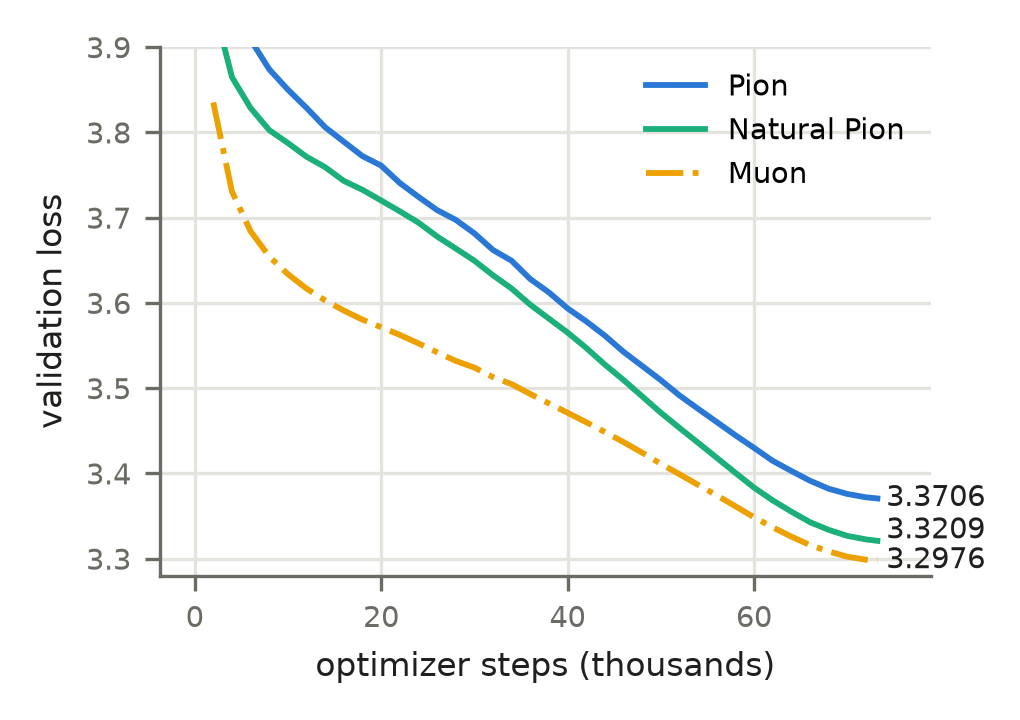
\includegraphics[width=\linewidth]{val_vs_steps.png}
\caption{Validation loss against optimizer steps on LLaMA-60M / C4 at Pion's full budget (73 242 steps, 9.6B tokens),
seed 0. Muon, which does not keep the spectrum, for reference.}\label{fig:val}
\end{figure}

Most optimizers for neural networks update a weight matrix additively, \(W \leftarrow W - \eta\,\Delta\),
and differ in how they shape \(\Delta\) from the gradient: Adam rescales it per coordinate, K-FAC and Shampoo
precondition it with Kronecker factors, and Muon replaces it with its orthogonal polar factor. Pion \citep{shi2026pion} takes a different
route: it updates \(W\) multiplicatively, by rotating it on both sides,
\[W \leftarrow R_{\mathrm{out}}\, W\, R_{\mathrm{in}}, \qquad R_{\mathrm{out}} \in O(m),\; R_{\mathrm{in}} \in O(n),\]
so the singular values of \(W\) are preserved throughout training. In particular, every weight keeps its initial
spectral norm, with no weight decay or norm constraint needed. Pion reports that this makes training stable and
competitive with Adam and Muon for LLM pretraining and finetuning.

Pion picks the rotation by steepest descent: it follows the gradient of the loss with respect to the two rotation
generators. Steepest descent depends on the metric, and Pion's metric treats every direction of rotation alike. Yet
the loss can be far more sensitive to some rotations of a matrix than to others. The classical
remedy is the natural gradient \citep{amari1998natural}, which measures steps by the Fisher information, the metric of
the model's output distribution. In the K-FAC approximation, we derive the natural gradient for Pion's rotations and
build on it an optimizer, \textbf{Natural Pion}.

Doing this directly runs into three obstacles. First, on the rotation generators the Fisher is not a Kronecker
product, so K-FAC's inverse does not apply; solved as a dense system, it costs \(O(n^6)\) per matrix. Second, the
natural gradient gives a good direction but a bad scale: at a fixed step size, its rotation angles differ by a factor
of \pn{angle_spread_fixed}{.1e} across the matrices. Third, the resulting rotations are about
\pn{ang_ratio_med}{.0f}x larger than Pion's, and at such angles Pion's truncated exponential no longer preserves the
spectrum.

\textbf{Result.} On LLaMA-60M trained on 9.6B tokens of C4, Pion's full budget, Natural Pion reaches Pion's losses in
\pn{budget_lo}{.2f}--\pn{budget_hi}{.2f}x fewer steps (Figure~\ref{fig:budget}). At full length it lowers the
validation loss from \pn{pion_full_best}{.4f} to \pn{v2_full}{.4f} (Figure~\ref{fig:val}), at
\pn{flops_60M_ratio}{.2f}x Pion's floating-point operations per step. Muon, which does not preserve the spectrum, is
still ahead, but Natural Pion closes about two thirds of Pion's gap to it (Section~\ref{sec:main}).

\textbf{Contributions.}

\begin{enumerate}
\def\labelenumi{\arabic{enumi}.}
\tightlist
\item
  \textbf{The Fisher on rotation generators, in closed form.} Under the K-FAC approximation, the Fisher on each side's
  rotations is \(F(X) = \tfrac12(SXA + AXS)\) (Proposition 1). The reason is simple: one token's rotation gradient is a
  bivector. \(F(X) = G\) is a generalized Lyapunov equation, which the classical simultaneous diagonalisation of the
  pencil \((A, S)\) solves exactly with one generalized eigendecomposition per side (Proposition 2).
\item
  \textbf{Direction from the Fisher, length from Pion.} We use only the direction of \(F^{-1}G\) and take the step
  length from Pion's RMS rule. With everything else fixed, this direction beats Pion's raw gradient by
  \pn{gain_fisher_mom}{.3f} in loss at 3 000 steps (Sections~\ref{sec:length} and~\ref{sec:ablations}).
\item
  \textbf{A retraction that preserves the spectrum at large angles.} We apply Cayley steps by scaling and squaring,
  computed by Newton--Schulz with matrix products only. This keeps the spectrum to \pn{rd_ns_delta_med}{.1e} of each
  matrix's scale; Pion's truncated exponential moves it by \pn{rd_trunc_med}{.1e} (Section~\ref{sec:retraction}).
\item
  \textbf{A fast implementation.} Refreshing the curvature every 25 steps, collecting statistics only before a refresh,
  batching, and lower precision before the rotation make the step \pn{speedup_vs_exact}{.1f}x faster than the exact
  form at the same loss (Algorithm~\ref{alg:1}, Section~\ref{sec:cost}, Appendix~\ref{sec:C}).
\end{enumerate}

Code, run records and every check script cited here are at \url{https://github.com/Max0072/NaturalPion}; paths in
typewriter type refer to that repository.

\section{Background}\label{sec:2}

\subsection{Pion: training by orthogonal equivalence}\label{sec:2.1}

Let \(W \in \mathbb{R}^{m \times n}\) be a weight matrix with loss gradient \(G = \partial L / \partial W\).
Pion parameterises an update by two skew-symmetric generators,
\(\Omega_{\mathrm{in}} \in \mathfrak{so}(n)\) and \(\Omega_{\mathrm{out}} \in \mathfrak{so}(m)\), and sets
\[W(\Omega) = e^{\Omega_{\mathrm{out}}}\, W\, e^{\Omega_{\mathrm{in}}}.\]
The derivative at \(\Omega = 0\) is \(\Omega_{\mathrm{out}} W + W \Omega_{\mathrm{in}}\). Write
\(\langle M, N \rangle = \operatorname{tr}(M^\top N)\) and \(\operatorname{skew}(M) = \tfrac12(M - M^\top)\).
For skew \(\Omega\), \(\langle M, \Omega\rangle = \langle \operatorname{skew}(M), \Omega\rangle\), so
\begin{gather*}
dL = \langle G W^\top, \Omega_{\mathrm{out}}\rangle + \langle W^\top G, \Omega_{\mathrm{in}}\rangle
\\ \Longrightarrow\quad
G_{\mathrm{in}} = \operatorname{skew}(W^\top G), \qquad G_{\mathrm{out}} = \operatorname{skew}(G W^\top)
\end{gather*}
are the gradients of the loss with respect to the two generators (the Riemannian gradient on
\(O(m) \times O(n)\) at the identity).

Pion steps along \(-G_{\mathrm{in}}\) and \(-G_{\mathrm{out}}\) with three further ingredients:

\begin{itemize}
\tightlist
\item
  \textbf{Lie-algebra momentum.} An exponential moving average of \(G_{\mathrm{in}}\) and \(G_{\mathrm{out}}\).
\item
  \textbf{RMS scaling.} The step is scaled so that the change it makes to \(W\),
  \(W\Omega_{\mathrm{in}} + \Omega_{\mathrm{out}} W\), has a target RMS (0.2 times the learning rate).
\item
  \textbf{A truncated exponential retraction} \(e^{\Omega} \approx I + \Omega + \Omega^2/2\).
\end{itemize}

Pion applies both rotations at every step (the \emph{bilateral} update); an alternating variant is slightly
worse at 60M. Only the 2-D weights inside the transformer blocks are rotated; embeddings, the output head and
normalization gains are trained by AdamW.

\subsection{The natural gradient and K-FAC}\label{sec:2.2}

For a model with predictive distribution \(p_\phi(y \mid x)\), the Fisher information
\(F = \mathbb{E}[\nabla_\phi \log p\, \nabla_\phi \log p^\top]\) defines a metric on parameter space. The
natural gradient \(F^{-1}\nabla L\) is the steepest-descent direction in that metric \citep{amari1998natural}:
\[-F^{-1}\nabla L \;\propto\; \arg\min_{\Delta}\; \langle \nabla L, \Delta\rangle
\quad \text{s.t.} \quad \tfrac12 \Delta^\top F \Delta \le r .\]
In a language model the samples in this expectation are tokens. For each token \(t\), a linear layer
\(y = Wx\) sees an input \(x_t\) and receives an output gradient \(\delta_t = \partial \ell_t / \partial y_t\); its
weight gradient is the average of the outer products \(\delta_t x_t^\top\). K-FAC \citep{martens2015kfac} assumes \(x\) and \(\delta\) are independent, which gives
\(F_W \approx A \otimes D\) with \(A = \mathbb{E}_t[x_t x_t^\top]\) and \(D = \mathbb{E}_t[\delta_t\delta_t^\top]\).
As an operator on matrices, \(F_W(Z) = D Z A\).

Strictly, the Fisher averages over outputs \(y\) sampled from the model. Like most K-FAC
implementations, we use the \textbf{empirical Fisher}: \(\delta_t\) is the gradient of the training loss at
the observed next token (Section~\ref{sec:ablations} compares it with the true Fisher).

\section{Method}\label{sec:3}

\subsection{The Fisher on rotation generators}\label{sec:fisher}

By Section~\ref{sec:2.1}, token \(t\)'s gradient with respect to \(\Omega_{\mathrm{in}} \in \mathfrak{so}(n)\) is
\(g_t = \operatorname{skew}(W^\top \delta_t\, x_t^\top)\). The (empirical) Fisher on \(\mathfrak{so}(n)\) is the second moment of
\(g_t\), the operator \(F_{\mathrm{in}}(X) = \mathbb{E}_t[\langle g_t, X\rangle\, g_t]\). As a matrix it has about
\(1.7\cdot10^{10}\) entries for \(n = 512\) and cannot even be stored. What makes it tractable is the form of \(g_t\).
With \(u_t = W^\top \delta_t\), the output gradient pulled back to the input space,
\[g_t = \tfrac12\big(u_t x_t^\top - x_t u_t^\top\big) = \tfrac12\, u_t \wedge x_t, \quad \langle g_t, X\rangle = u_t^\top X x_t,\]
so \(g_t\) is a bivector, and its pairing with a skew \(X\) is a single bilinear form. Expanding the second moment and
factorising it as K-FAC does leaves two \(n \times n\) matrices. On the output side, \(\delta_t\) and \(v_t = W x_t\) play the
roles of \(u_t\) and \(x_t\).

\textbf{Proposition 1 (Fisher on the generators).} Under the K-FAC independence assumption, and treating
the two sides separately,
\[F_{\mathrm{in}}(X) = \tfrac12\big(S X A + A X S\big), \qquad S = W^\top D W,\]
\[F_{\mathrm{out}}(Y) = \tfrac12\big(D Y V + V Y D\big), \qquad V = W A W^\top,\]
for \(X \in \mathfrak{so}(n)\), \(Y \in \mathfrak{so}(m)\). Both operators are self-adjoint and positive
semi-definite on the skew matrices: \(\langle Z, SXA + AXS\rangle\) is symmetric in \(X\) and \(Z\), and
\(\langle X, F_{\mathrm{in}}(X)\rangle = \mathbb{E}[(u^\top X x)^2] \ge 0\) before the factorisation and
\(\tfrac12\langle X, SXA + AXS\rangle = \|S^{1/2} X A^{1/2}\|_F^2 \ge 0\) after it. The derivation is in Appendix~\ref{sec:derivation}.

\textbf{Relation to K-FAC.} This operator is K-FAC itself, written on the rotation generators. A generator
changes \(W\) by \(J(\Omega) = W\Omega\), and the adjoint of this map is \(J^*(M) = \operatorname{skew}(W^\top M)\).
Pulling K-FAC's Fisher on \(W\), \(F_W(Z) = DZA\), back through \(J\) gives
\begin{align*}
J^* F_W J(X) &= \operatorname{skew}(W^\top D\, W X\, A) \\
&= \operatorname{skew}(S X A) = \tfrac12\big(SXA + AXS\big),
\end{align*}
which is Proposition 1. The result is not a Kronecker product, so K-FAC's inverse \(D^{-1} Z A^{-1}\) does not
apply; Section~\ref{sec:inversion} inverts it instead.

\textbf{What is approximated.} Three things: \(x\) and \(\delta\) are treated as independent, as in K-FAC; the two
sides and the layers are treated separately; and the empirical Fisher stands in for the true one
(Section~\ref{sec:2.2}). The rest is exact algebra, which Appendix~\ref{sec:derivation} also checks numerically; how
far K-FAC is from the exact curvature along our step is measured in Section~\ref{sec:length}.

\subsection{Exact inversion}\label{sec:inversion}

\(F_{\mathrm{in}}\) acts on a space of dimension \(n(n-1)/2\). Solving \(F_{\mathrm{in}}(X) = G\) as a dense
linear system costs \(O(n^6)\), about \(10^{15}\) operations for \(n = 512\), for every matrix at every refresh.
Nor can it be inverted factor by factor like \(X \mapsto SXA\), whose inverse is \(S^{-1} G A^{-1}\): the sum of
the two orderings does not factor unless \(S\) and \(A\) commute. A congruence diagonalises it nonetheless, at
\(O(n^3)\): \(SXA + AXS = 2G\) is a generalized Lyapunov equation, and simultaneous diagonalisation of the pencil
\((A, S)\) is the standard way to solve it \citep{golub2013matrix,simoncini2016computational}. We state the solution for
completeness.

\textbf{Proposition 2 (Inversion).} Let \(A \succ 0\) and \(S \succeq 0\), and let \(P\) solve the generalized
eigenproblem \(P^\top A P = I\), \(P^\top S P = \Lambda = \operatorname{diag}(\lambda)\), with \(\lambda_i + \lambda_j > 0\)
for all \(i \neq j\) (the diagonal of a skew matrix is zero). For skew \(G\), the unique skew solution of \(F_{\mathrm{in}}(X) = G\) is
\[X = P\, \big[ (P^\top G P) \oslash K \big]\, P^\top, \qquad K_{ij} = \tfrac12(\lambda_i + \lambda_j),\]
where \(\oslash\) is elementwise division.

\emph{Proof.} Substitute \(X = P\tilde X P^\top\):
\(P^\top (SXA + AXS) P = (P^\top S P)\, \tilde X\, (P^\top A P) + (P^\top A P)\, \tilde X\, (P^\top S P) = \Lambda \tilde X + \tilde X \Lambda\).
So \(F_{\mathrm{in}}(X) = G\) becomes \(\tfrac12(\lambda_i + \lambda_j)\, \tilde X_{ij} = (P^\top G P)_{ij}\). Since
\(P^\top G P\) is skew, so are \(\tilde X\) and \(X\). \(P\) is invertible, so the solution is unique. \(\square\)

The same construction applies to the output side, with \(A\) replaced by \(D\) and \(S\) by \(V = WAW^\top\).
\(A\) and \(D\) need not be positive definite; the floor below makes them so, as the proposition requires.

\textbf{Computation.} We compute \(P = A^{-1/2} Q\), with \(Q\) the eigenvectors of \(A^{-1/2} S A^{-1/2}\). The
symmetric root, rather than a Cholesky factor, exposes the eigenvalues so they can be floored.

\textbf{Regularisation.} A single relative floor: every spectrum the solve uses (\(A\), \(S\), \(\Lambda\) on the
input side; \(D\), \(V\), \(\Lambda\) on the output side) is raised to at least \(\varepsilon \lambda_{\max}\), with
\(\varepsilon = 10^{-3}\). Unlike an additive shift, a floor leaves every eigenvalue above it unchanged.

\textbf{Cost.} One generalized eigendecomposition per side, \(O(n^3)\), at every refresh (Algorithm~\ref{alg:1} amortises it); applying
\(F^{-1}\) between refreshes costs four matrix products per side.

\subsection{Step length}\label{sec:length}

The natural gradient gives a direction \(X = F^{-1}G\), but its scale is a poor guide. At a fixed step size, the
rotation angle it produces differs by a factor of \pn{angle_spread_fixed}{.1e} across the rotated matrices (90th over
10th percentile, Section~\ref{sec:ablations}). The scale is also where K-FAC is least reliable: along our step, its
curvature is \pn{kfac_vs_exact}{.2g} of the exact per-token curvature on a trained model
(\texttt{scripts/probes/paper\_checks.py}). So we keep the direction and take the length from Pion: the coefficient
\(c\) sets the RMS of the change the step makes to \(W\) to the scheduled \(\theta_t\),
\[c_t = \theta_t\, \frac{\sqrt{mn}}{\|W X_{\mathrm{in}} + X_{\mathrm{out}} W\|_F},\]
the same rule Pion applies to its raw generators. Since \(c\) is set per matrix, the Fisher's scale across matrices is
discarded. What the Fisher still decides is the direction within each matrix and, since both sides share \(c\), the
balance between its two sides. To first order in the angle, each rotation plane then turns in proportion to the
corresponding singular value of \(X\). \(\theta_t\) follows a cosine schedule from a peak \(\theta_0\). Section~\ref{sec:ablations} compares this rule
with fixing the rotation angle (\(c = \theta/\sigma(X)\)) and with measuring the length in the Fisher metric.

\textbf{Proposition 3 (Angle of a Cayley step).} Let \(X\) be skew with largest singular value \(\sigma\) and
\(c > 0\). The rotation \(R = \big(I + \tfrac c2 X\big)^{-1}\big(I - \tfrac c2 X\big)\) turns its planes by
the angles \(2\arctan(c\,\sigma_j/2)\), where \(\sigma_j\) are the singular values of \(X\). Its largest
angle is \(2\arctan(c\sigma/2) = c\sigma + O((c\sigma)^3)\).

\emph{Proof.} A real skew matrix has eigenvalues \(\pm i\sigma_j\), in planes that are mutually orthogonal.
On such a plane \(R\) acts by \((1 - ic\sigma_j/2)/(1 + ic\sigma_j/2) = e^{-2i\arctan(c\sigma_j/2)}\).
\(\square\)

Under the RMS rule \(c\sigma\) is not fixed: a plane that carries little of \(W\) barely moves it, so it may turn
far. At the worst logged step, early in training, a tenth of the matrices turn their fastest plane by
\pn{ang_p90_max}{.2f} rad or more, and the retraction has to handle this. Over the first thousand steps, where both are
measured, the median angle is \pn{ang_ratio_med}{.1f} times Pion's (range \pn{ang_ratio_min}{.1f} to
\pn{ang_ratio_max}{.1f}; Figure~\ref{fig:angles}).

\begin{figure}[t]
\centering
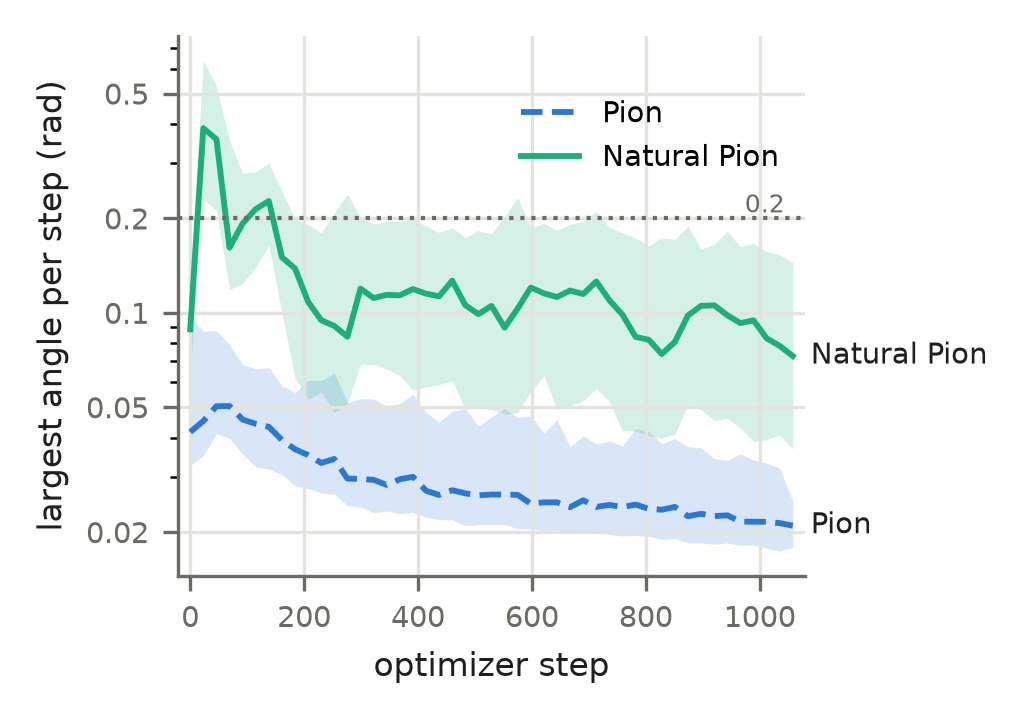
\includegraphics[width=\linewidth]{angles.png}
\caption{Largest rotation angle per rotated matrix and step: median
over the matrices, band from the 10th to the 90th percentile, log scale.
First \pn{pion_angle_steps}{,.0f} steps, where both were recorded and the
learning rate is near its peak. Natural Pion at 3 000 steps, seed 0; Pion
at lr \(10^{-3}\) on a 3 840-step schedule
(\texttt{scripts/probes/pion\_angles.py}).
Dotted: 0.2, above which the
squared Cayley retraction splits the step (Section~\ref{sec:retraction}).}\label{fig:angles}
\end{figure}

\subsection{Retraction: the squared Cayley map}\label{sec:retraction}

\textbf{Proposition 4.} For skew \(\Psi\), the Cayley map \(R = (I + \Psi)^{-1}(I - \Psi)\) is orthogonal
for every scale of \(\Psi\). Hence \(R_{\mathrm{out}} W R_{\mathrm{in}}\) has exactly the singular values
of \(W\). The degree-2 truncated exponential \(T = I + \Psi + \Psi^2/2\) satisfies
\(T^\top T = I + \Psi^4/4\).

\emph{Proof.} The eigenvalues of a real skew \(\Psi\) are \(\pm i\sigma_j\), so those of \(I + \Psi\) are
\(1 \pm i\sigma_j \neq 0\) and \(I + \Psi\) is invertible. \(I + \Psi\) and \(I - \Psi\) commute, and
\((I \pm \Psi)^\top = I \mp \Psi\), so
\(R^\top R = (I + \Psi)(I - \Psi)^{-1}(I + \Psi)^{-1}(I - \Psi) = I\). For \(T\), expand with
\(\Psi^\top = -\Psi\): the odd and quadratic terms cancel, leaving \(\Psi^4/4\). \(\square\)

\textbf{What the retraction must do.} It must stay orthogonal to round-off at every angle, on every matrix and every
step. Pion's angles are smaller and more uniform: the median over the rotated matrices is \pn{pion_angle_block_median}{.2g}
rad per step (p90/p10 \pn{pion_angle_spread}{.1f}), the largest \pn{pion_angle_max}{.2g}
(\texttt{scripts/probes/pion\_angles.py}, first \pn{pion_angle_steps}{,.0f} steps). By Proposition 4, one
truncated-exponential step at angle \(a\) changes a singular value by \(\sqrt{1 + a^4/4} - 1 \approx a^4/8\). That is
about \pn{trunc_err_pion}{.0e} per step at Pion's typical angle, but \pn{trunc_at_ang_p50_med}{.0e},
\pn{trunc_at_ang_p90_med}{.0e} and \pn{trunc_at_ang_p90_max}{.0e} at ours (3 000 steps; the run's median of the 50th and
90th percentiles over the matrices, and the largest 90th percentile).

\textbf{Cayley by Newton--Schulz.} The Cayley map needs a linear solve: \(\mathrm{Cay} = 2(I + \Psi)^{-1} - I\) with
\(\Psi = \tfrac c2 X\). Newton--Schulz computes \((I + \Psi)^{-1}\) with matrix products only,
\(Z \leftarrow Z(2I - (I + \Psi)Z)\) from \(Z_0 = I - \Psi\). After two iterations the error is
\(2(I+\Psi)^{-1}\Psi^8\): the largest entry of \(R^\top R - I\) is \pn{ns_err_02}{.0e} at angle \(a = c\|X\|_2 = 0.2\), \pn{ns_err_04}{.0e} at 0.4, \pn{ns_err_08}{.0e} at 0.8 (fp64).

In fp32 this standard form is biased. Entries close to 1 lose their low bits, always in the same direction, so
\(\|W\|_F^2\), which a rotation should keep, grows by a median \pn{diag_ns_step}{.1e} per training step (exact solve:
\pn{diag_cayley_step}{.1e}; \texttt{scripts/probes/ns\_diag.py}). We therefore iterate on \(\Phi = Z - I\), from
\(\Phi_0 = -\Psi\): residual \(E = \Psi + \Phi + \Psi \Phi\), update \(\Phi \leftarrow \Phi - E - \Phi E\), rotation
\(I + 2\Phi\). No entry is then close to 1, and the number of products is the same. Appendix~\ref{sec:impl} checks the bias over random rotations.

\textbf{Scaling and squaring.} Two iterations reach fp32 accuracy only up to an angle of about 0.2, and the RMS rule
takes larger steps. Natural Pion therefore halves the step's largest angle (estimated from \(\sigma\),
Appendix~\ref{sec:C.5}) \(q\) times until it is at most 0.2, runs the two iterations on \(\Psi / 2^q\), and squares the
result \(q\) times. The squaring uses the same correction form, \(H \leftarrow 2H + H^2\) for \(R = I + H\), so again
nothing is rounded near 1. Each squaring costs one product, less than the extra iterations or the exact solve it
replaces (\texttt{scripts/probes/cayley\_speed.py}).

The result, \(R = \mathrm{Cay}(cX / 2^q)^{2^q}\), is no longer the Cayley transform of \(cX\). Since Cayley is the
\([1/1]\) Padé approximant of the exponential, it is the scaling-and-squaring method for the matrix exponential
\citep{higham2005scaling} with that approximant, an approximation of the geodesic step on \(O(n)\). We call it the
squared Cayley retraction. On the plane of singular value \(\sigma_j\) it turns by
\(2^{q+1}\arctan(c\sigma_j / 2^{q+1})\); with \(y = c\sigma_j/2^q \le 0.2\), this matches the exponential's angle
\(c\sigma_j\) to a relative \(y^2/12 \le 1/300\) at any step length (Proposition 3 applies to each factor, not to \(R\)).
With exact Cayley factors \(R\) is orthogonal, because a diagonal Padé approximant maps skew matrices to orthogonal ones;
a truncated Taylor series, Pion's approximation of the same exponential, does not (Proposition 4). In practice each
factor carries the error of its Newton--Schulz inverse, and the squarings multiply it by up to \(2^q\). In training the
spectrum moves by \pn{rd_ns_delta_med}{.1e} of its scale over 3 000 steps (Table~\ref{tab:2}). For most of the run the
90th percentile of the angle is below 0.2 (median \pn{ang_p90_med}{.2f} rad), so the squarings matter mainly early in
training.

\begin{table*}[t]
\centering\small
\caption{Retractions: Natural Pion (Algorithm~\ref{alg:1}) with each, seed 0. First column:
change of \(\|W\|_F^2\) over 200 steps of a bare \(1376 \times 1376\)
rotation at angle 0.05 (\texttt{scripts/probes/ns\_rounding.py}). Drift:
\(\max_i |s_i - s_i^0| / \max_i s_i^0\) after 3 000 training steps,
median / worst over the rotated matrices
(\texttt{scripts/probes/retraction\_drift.py}). --: not run.}\label{tab:2}
\begin{tabularx}{\linewidth}{>{\raggedright\arraybackslash}Xlllll}
\toprule
retraction & \(\Delta\|W\|_F^2\), bare matrix & val, 3 000 steps & val, 15 000 steps & drift & s / step \\
\midrule
Cayley, exact solve & \pn{rnd_cayley_0.05}{+.1e} & \pn{ret_cayley_3000}{.4f} & -- & \pn{rd_cayley_med}{.1e} / \pn{rd_cayley_max}{.1e} & \pn{ret_cayley_sps}{.3f} \\
Cayley, Newton--Schulz (standard form, iterations growing with the
angle, no squaring) & \pn{rnd_ns_0.05}{+.1e} & \pn{ret_ns_3000}{.4f} & -- & \pn{rd_ns_med}{.1e} / \pn{rd_ns_max}{.1e} & \pn{ret_ns_sps}{.3f} \\
squared Cayley (Natural Pion) & \pn{rnd_ns_delta_0.05}{+.1e} & \pn{v2_3000_s0}{.4f} & \pn{v2_15000_s0}{.4f} & \pn{rd_ns_delta_med}{.1e} / \pn{rd_ns_delta_max}{.1e} & \pn{m_sps}{.3f} \\
truncated exponential, degree 2 (Pion's) & -- & \pn{ret_trunc_3000}{.4f} & \pn{ret_trunc_15000}{.4f} & \pn{rd_trunc_med}{.1e} / \pn{rd_trunc_max}{.1e} & \pn{ret_trunc_sps}{.3f} \\
\bottomrule
\end{tabularx}
\end{table*}

At 3 000 steps the validation losses of the four retractions lie within \pn{ret_loss_range}{.3f} of each other (one
run each; the method's four seeds span \pn{v2_3000_range}{.3f}); at 15 000 steps the truncated exponential is
\pn{ret_trunc_15k_d}{+.4f} from the method. So the retraction decides the spectrum, not the loss: the squared Cayley
retraction moves it by \pn{rd_ns_delta_med}{.1e}, the others by \pn{rd_cayley_med}{.1e} to \pn{rd_ns_med}{.1e}.

\textbf{Precision.} The retraction must run in true fp32: over 200 exact Cayley steps at angle \(10^{-2}\) on a
\(512 \times 1376\) matrix, TF32 moves a singular value by up to \pn{tf32_drift}{.2\%} (relative), fp32 by \pn{fp32_drift_200}{.3\%}.

\subsection{The algorithm}\label{sec:algorithm}

Algorithm~\ref{alg:1} is Natural Pion as run in every experiment. Like K-FAC with its inverse
\citep[][Sec.~13]{martens2015kfac}, it amortises the bases: they are recomputed every \(T_{\mathrm{fac}} = 25\) steps,
and \(A\) and \(D\) are accumulated only in the 6 steps before each refresh, since nothing else reads them.
\(F^{-1}\), the step's scale and the retraction run as one batched call per matrix shape, and the largest angle
\(\sigma\) comes from a warm-started power iteration. The \emph{exact form}, our reference in Section~\ref{sec:cost} and
Appendix~\ref{sec:C}, recomputes everything at every step (\(T_{\mathrm{fac}} = 1\), \(A\) with EMA 0.95 and \(D\) with
0.5, both every step) and uses the exact Cayley solve \(\mathrm{Cay}(cX) = (I + \tfrac c2 X)^{-1}(I - \tfrac c2 X)\).

\begin{algorithm*}[t]
\caption{Natural Pion, for one rotated matrix \(W \in \mathbb{R}^{m\times n}\) (all of them processed alike, batched by shape).}\label{alg:1}
\vspace{-0.5em}
\scriptsize
\begin{verbatim}
state:  A, D: EMAs (0.5, fp32) of x x^T and d d^T;  M_in, M_out: momentum (beta1 = 0.9), zero at start;
        bases (P, lambda) per side;  eps = 1e-3,  T_fac = 25
every step t:
    theta_t <- theta_min + (theta_0 - theta_min)(1 + cos(pi t / T)) / 2     cosine; theta_min = theta_0 / 100
    if t is one of the 6 steps before a refresh:                one A per input tensor; bf16 inputs, fp32 sums
        forward:  A <- 0.5 A + 0.5 mean_tokens(x x^T)
        backward: D <- 0.5 D + 0.5 mean_tokens(d d^T)            d = per-token output gradient
    if t is a refresh step (every T_fac steps):                 the bases (Prop. 2); spectra floored at eps * max
        (P_in, lambda_in)   <- gen_eig(A, W^T D W)
        (P_out, lambda_out) <- gen_eig(D, W A W^T)
    G_in  <- skew(W^T G);   G_out <- skew(G W^T)
    M_in  <- beta1 M_in  + (1 - beta1) G_in;   M_out <- beta1 M_out + (1 - beta1) G_out
    X_in  <- P_in  [ (P_in^T  M_in  P_in)  / K_in  ] P_in^T     K_ij = (lambda_i + lambda_j)/2; products in bf16
    X_out <- P_out [ (P_out^T M_out P_out) / K_out ] P_out^T
    c     <- theta_t sqrt(m n) / ||W X_in + X_out W||_F          Pion's RMS rule
    sigma <- max(||X_in||_2, ||X_out||_2)                        warm power iteration (2 steps; 50 after refresh)
    q     <- smallest q >= 0 with c sigma / 2^q <= 0.2
    W     <- SqCay(c X_out) W SqCay(c X_in)          in fp32; SqCay(cX) = Cay(cX / 2^q)^(2^q),
                                                     each Cay by 2 Newton-Schulz steps in Z - I (Sec. 3.4)
\end{verbatim}
\end{algorithm*}

As in Pion, embeddings, the output head and normalization gains use AdamW. The rotated matrices get no weight
decay: a rotation cannot change their norm.

Under the RMS rule, a constant factor in \(A\) or \(D\) (such as autograd's \(1/N\)) cancels in \(cX\); the Fisher-norm and
quadratic-model rules and the damping of Section~\ref{sec:ablations} need \(D\) at its true scale (Appendix~\ref{sec:impl}).

\section{Experiments}\label{sec:experiments}

\subsection{Setup}\label{sec:setup}

\textbf{Model and data.} A LLaMA-style model of 60M parameters (hidden 512, 8 layers, 8 heads, SwiGLU FFN, RoPE,
RMSNorm, T5 vocabulary) on C4, sequence length 256, batch 512 sequences (131 072 tokens per step), for 73 242 steps =
9.6B tokens: Pion's 60M budget. The 56 matrices inside the blocks (\pn{rotated_share}{.1\%} of parameters) are rotated;
the rest are trained by AdamW (lr \(8\cdot10^{-3}\), betas (0.9, 0.95), weight decay 0.1), the same for every method. The metric is
validation loss, token cross-entropy on held-out C4 in nats; each run uses one NVIDIA RTX PRO 6000 Blackwell.
Appendix~\ref{sec:B} gives the full setup (Table~\ref{tab:setup}) and hyperparameters (Table~\ref{tab:hyper}).

\textbf{Baseline.} Pion's rotation update in its published settings: Lie momentum 0.9, RMS scale 0.2, truncated
exponential, bilateral update, cosine schedule. The Pion paper chose lr \(10^{-3}\) from
\(\{10^{-4}, 5\cdot10^{-4}, 10^{-3}, 5\cdot10^{-3}, 10^{-2}\}\). Since Natural Pion's scale is chosen per budget, so is
Pion's lr: from 15 000 steps on we take the better of \(10^{-3}\) and \(2\cdot10^{-3}\) (seed 0) at every budget.
Table~\ref{tab:4} (Appendix~\ref{sec:B}) shows a wider grid at 3 840 and 19 200 steps.

All comparisons use one code base and one data pipeline (Muon's run below uses a copy of it). In our setting Pion
ends at a training loss of \pn{pion_full_train}{.4f} (mean over the last 2 000 steps; validation \pn{pion_full}{.4f}).
The Pion paper reads 3.3575 off its own training curve in Megatron-LM \citep{shoeybi2019megatron}. A single batch's
training loss varies by \pn{pion_train_batch_sd}{.3f} here, so the two numbers are not directly comparable, and we
compare within our setting only.

\textbf{Natural Pion.} Algorithm~\ref{alg:1}, Lie momentum 0.9, floor \(\varepsilon = 10^{-3}\). Every schedule of
every method, \(\theta\) and AdamW's lr alike, is a cosine down to 1\% of its peak (for Pion at lr \(10^{-3}\),
\(10^{-5}\)). The peak RMS scale \(\theta_0\) is chosen per horizon on a grid of factors of two: \pn{scale_3000}{.1e} at 3 000 steps,
\pn{scale_9000}{.1e} at 9 000, \pn{scale_15000}{.1e} at 15 000 and \pn{scale_30000}{.1e} at 30 000; the longer budgets keep the
30 000-step choice. These peaks are close to Pion's own target, \(0.2 \cdot \mathrm{lr} = 2\cdot10^{-4}\) to
\(4\cdot10^{-4}\): per step, Natural Pion changes \(W\) by about as much as Pion does, so its gain comes from the
direction of the step, not from a larger one.

\subsection{Main result}\label{sec:main}

\begin{table}[t]
\centering\small
\caption{Equal number of steps (seed 0 unless marked). Pion at the
better of lr \(10^{-3}\) and \(2\cdot10^{-3}\) at each budget (Section~\ref{sec:setup}); at 3 000 steps \(10^{-3}\). Gap = val(Pion) - val(Natural Pion).}\label{tab:5}
\begin{tabularx}{\linewidth}{>{\raggedright\arraybackslash}Xlll}
\toprule
steps & Pion & Natural Pion & gap \\
\midrule
3 000 (mean of 4 seeds) & \pn{pion3000_mean}{.4f} & \pn{v2_3000_mean}{.4f} & \pn{v2_gap3000}{.3f} \\
15 000 & \pn{pion15k_best}{.4f} & \pn{v2_15000_s0}{.4f} & \pn{v2_gap15k}{.3f} \\
73 242 (full length) & \pn{pion_full_best}{.4f} & \pn{v2_full}{.4f} & \pn{v2_gap_full}{.3f} \\
\bottomrule
\end{tabularx}
\end{table}

Figure~\ref{fig:val} shows the full-length curves. At 3 000 steps the smallest per-seed gap is
\pn{v2_gap3000_min}{.3f}. Seed 0 was also used to choose Natural Pion's scale; over seeds 1--3 alone its mean is
\pn{v2_3000_mean13}{.4f} at 3 000 steps and \pn{v2_15000_mean13}{.4f} at 15 000.

\textbf{Muon, for reference.} Muon \citep{jordan2024muon}, which does not preserve the spectrum, in the Pion authors'
configuration (lr \(10^{-3}\), same AdamW and schedule; micro-batch 512) reaches \pn{muon_full}{.4f} at full length:
\pn{muon_gap_full}{.3f} below Pion and \pn{muon_gap_np}{.3f} below Natural Pion. The Pion paper also reports Muon ahead of
Pion (its Table 1, 1.3B). Natural Pion thus closes \pn{gap_closed_frac}{.0\%} of Pion's gap to Muon, and
\pn{aw_gap_closed_frac_best}{.0\%} against Pion at its best full-length AdamW learning rate (Table~\ref{tab:5b}). Muon is not
re-tuned here, so a tuned Muon would lower that share; how much of the remaining gap is the price of preserving the
spectrum, we do not know.

\textbf{AdamW at full length.} AdamW's lr (embeddings, head, norms) was chosen at 3 000 and 15 000 steps. At full
length, the best of the three values in Table~\ref{tab:5b} is \pn{aw_pion_best_lr}{.0e} for Pion and
\pn{aw_np_best_lr}{.0e} for Natural Pion, \pn{aw_pion_gain}{.3f} and \pn{aw_np_gain}{.3f} better than \(8\cdot10^{-3}\).
The gap stays between \pn{aw_gap_min}{.3f} and \pn{aw_gap_max}{.3f} (seed 0; Pion at the better of lr \(10^{-3}\) and
\(2\cdot10^{-3}\) for each AdamW lr).

\begin{table}[t]
\centering\small
\caption{Full length, by AdamW lr.}\label{tab:5b}
\begin{tabularx}{\linewidth}{>{\raggedright\arraybackslash}Xlll}
\toprule
AdamW lr & Pion & Natural Pion & gap \\
\midrule
\(10^{-3}\) & \pn{aw_pion_1e-3}{.4f} & \pn{aw_np_1e-3}{.4f} & \pn{aw_gap_1e-3}{.3f} \\
\(4\cdot10^{-3}\) & \pn{aw_pion_4e-3}{.4f} & \pn{aw_np_4e-3}{.4f} & \pn{aw_gap_4e-3}{.3f} \\
\(8\cdot10^{-3}\) (the rest of the paper) & \pn{aw_pion_8e-3}{.4f} & \pn{aw_np_8e-3}{.4f} & \pn{aw_gap_8e-3}{.3f} \\
\bottomrule
\end{tabularx}
\end{table}

\subsection{Steps to reach Pion's loss}\label{sec:budget}

Every run here has its own full cosine schedule ending at its budget \(B\), so no loss is read off the middle of a
schedule. For each method we fit the final validation loss as \(L(B) = a + bB^{-\gamma}\) (\pn{budget_n_pion}{} Pion
budgets, \pn{budget_n_np}{} Natural Pion budgets, four seeds at 3 000 and 15 000 steps; worst residual
\pn{budget_resid}{.4f}). The saving at Pion's loss \(L\) is \(B_{\mathrm{Pion}} / B_{\mathrm{NP}}(L)\), with
\(B_{\mathrm{NP}}\) taken from the fit or by linear interpolation in \(\log B\) between Natural Pion's budgets
(\texttt{scripts/analysis/budget\_fit.py}). Figure~\ref{fig:budget} shows both fits.

\begin{table}[t]
\centering\small
\caption{Steps saved at Pion's loss (mean over seeds where there are
four): fit / interpolation.}\label{tab:6}
\begin{tabularx}{\linewidth}{>{\raggedright\arraybackslash}Xll}
\toprule
Pion steps & Pion val & saving \\
\midrule
15 000 & \pn{budget_15000_L}{.4f} & \pn{budget_15000_pow}{.2f} / \pn{budget_15000_int}{.2f} \\
19 200 & \pn{budget_19200_L}{.4f} & \pn{budget_19200_pow}{.2f} / \pn{budget_19200_int}{.2f} \\
30 000 & \pn{budget_30000_L}{.4f} & \pn{budget_30000_pow}{.2f} / \pn{budget_30000_int}{.2f} \\
45 000 & \pn{budget_45000_L}{.4f} & \pn{budget_45000_pow}{.2f} / \pn{budget_45000_int}{.2f} \\
73 242 & \pn{budget_73242_L}{.4f} & \pn{budget_73242_pow}{.2f} / \pn{budget_73242_int}{.2f} \\
\bottomrule
\end{tabularx}
\end{table}

Pion's targets use its better lr of \(10^{-3}\) and \(2\cdot10^{-3}\) at each budget (Section~\ref{sec:setup}). The gap
in loss at equal steps shrinks with the budget (\pn{v2_gap3000}{.3f}, \pn{v2_gap15k}{.3f} and \pn{v2_gap_full}{.3f} at
3 000, 15 000 and 73 242 steps, Table~\ref{tab:5}) because both curves flatten. Measured in steps, the advantage does
not shrink: \pn{budget_15000_pow}{.2f}x at 15 000 steps, \pn{budget_73242_pow}{.2f}x at full length.

\begin{figure}[t]
\centering
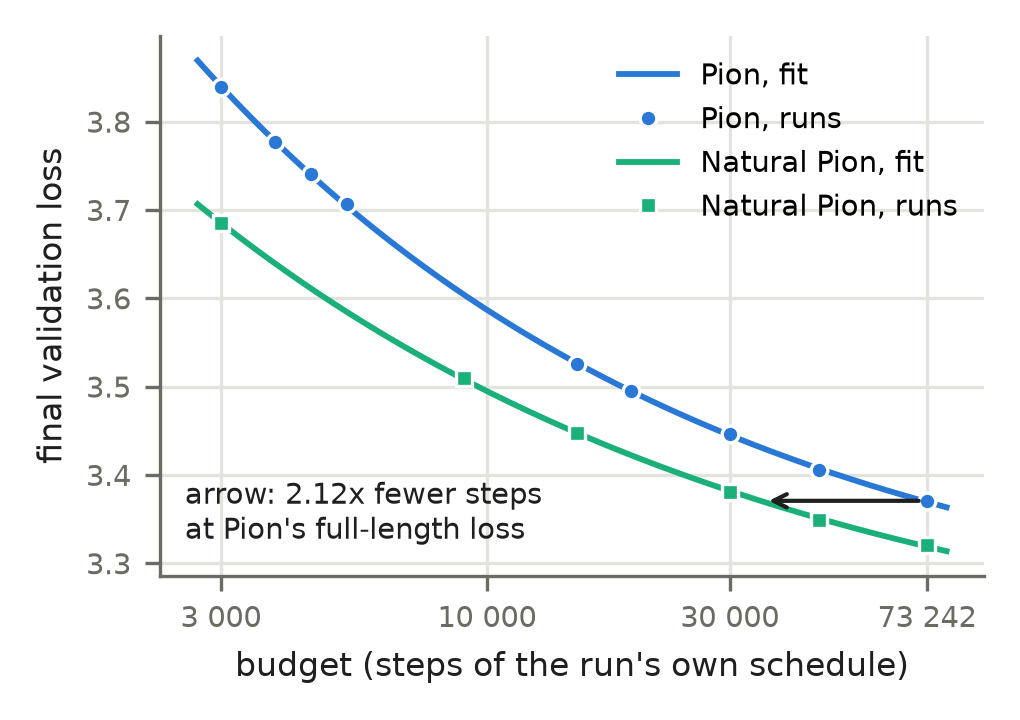
\includegraphics[width=\linewidth]{budget_fit.png}
\caption{Final validation loss of every full-schedule run against its
budget, with the fit \(L(B) = a + bB^{-\gamma}\) of each method; at 3
000 and 15 000 steps the mean of four seeds. The arrow is the saving at
Pion's full-length loss.}\label{fig:budget}
\end{figure}

\textbf{Equal wall-clock time.} A Natural Pion step takes \pn{v2_ratio}{.2f}x Pion's (Section~\ref{sec:cost}), so in
the time of Pion's \(B\) steps Natural Pion takes \(B/\pn{v2_ratio}{.2f}\). Read off the budget curve above (estimates,
not separate runs), the gap to Pion at Pion's full-length wall-clock time is \pn{eqt_73242_gap}{.3f} (fit;
\pn{eqt_73242_gap_int}{.3f} by interpolation), \pn{eqt_19200_gap}{.3f} at the time of 19 200 steps, and
\pn{eqt_3840_gap}{.3f} at the time of 3 840 steps.

\subsection{Ablations}\label{sec:ablations}

Each ablation changes one thing in Natural Pion (Algorithm~\ref{alg:1}) at 3 000 steps, seed 0. The reference is the
method itself: RMS scale \pn{scale_3000}{.1e}, Lie momentum 0.9, floor \(10^{-3}\) (\pn{v2_3000_s0}{.4f}). ``Best'' means
the best over a grid of that row's step-size parameter.

\textbf{The direction: natural gradient against the raw generator.} Only \(X = F^{-1}G\) against \(X = G\) changes;
the length rule, retraction and schedule are the same, each at the best scale of its grid.

\begin{table}[t]
\centering\small
\caption{The direction. Pion at 3 000 steps, seed 0: \pn{pion3000_s0}{.4f}.}\label{tab:7}
\begin{tabularx}{\linewidth}{>{\raggedright\arraybackslash}Xll}
\toprule
 & no momentum & Lie momentum 0.9 \\
\midrule
\(X = F^{-1}G\) & \pn{dir_fisher_nomom}{.4f} & \pn{dir_fisher_mom}{.4f} \\
\(X = G\) & \pn{dir_raw_nomom}{.4f} & \pn{dir_raw_mom}{.4f} \\
gain from \(F^{-1}\) & \pn{gain_fisher_nomom}{.3f} & \pn{gain_fisher_mom}{.3f} \\
\bottomrule
\end{tabularx}
\end{table}

\textbf{The length.} Only the length rule changes, each at the best \(\theta\) of its grid. The last column is the
spread of the realised rotation angle across the rotated matrices (90th over 10th percentile, median over the steps
after 1 000). In the quadratic-model and Fisher-norm rules, \(F\) is the Fisher at the current \(W\) with the current
statistics. With momentum, \(X = F^{-1}M\), so with a fresh basis \(\langle X, FX\rangle = \langle M, X\rangle\) and the
quadratic-model ratio is \(\langle G, X\rangle / \langle M, X\rangle\). It differs from a fixed \(c\) only where the
current gradient disagrees with the momentum or the basis has gone stale.

\begin{table}[t]
\centering\small
\caption{The length rule.}\label{tab:8}
\begin{tabularx}{\linewidth}{>{\raggedright\arraybackslash}Xll}
\toprule
length rule & val & angle spread \\
\midrule
RMS of the induced change, as in Pion (the method) & \pn{len_rms}{.4f} & \pn{angle_spread_rms}{.1e} \\
rotation angle: \(c = \theta/\sigma(X)\), \(X = F^{-1}M\) & \pn{len_angle}{.4f} & \pn{angle_spread_spectral}{.1e} \\
quadratic-model ratio,
\(c = \theta \min(1, \langle G, X\rangle / \langle X, FX\rangle)\) & \pn{len_quad}{.4f} & \pn{angle_spread_quad}{.1e} \\
Fisher norm, \(c = \theta / \sqrt{\langle X, FX\rangle}\) & \pn{len_fisher}{.4f} & \pn{angle_spread_fisher}{.1e} \\
fixed, \(c = \theta\) & \pn{len_fixed}{.4f} & \pn{angle_spread_fixed}{.1e} \\
rotation angle before \(F^{-1}\): \(c = \theta/\sigma(M)\) & \pn{len_before}{.4f} & \pn{angle_spread_before}{.1e} \\
\bottomrule
\end{tabularx}
\end{table}

Over four seeds, each at the best \(\theta\) of its grid, the RMS rule minus the angle rule is \pn{rms_gap_s0}{+.3f},
\pn{rms_gap_s1}{+.3f}, \pn{rms_gap_s2}{+.3f} and \pn{rms_gap_s3}{+.3f}: the two are within noise of each other, and we keep
Pion's rule.

\textbf{Regularisation of the Fisher.} The default is a relative floor \(\varepsilon = 10^{-3}\) (\pn{v2_3000_s0}{.4f}).

\begin{table}[t]
\centering\small
\caption{Regularisation of the Fisher.}\label{tab:9}
\begin{tabularx}{\linewidth}{>{\raggedright\arraybackslash}Xllll}
\toprule
floor \(\varepsilon\) (no damping) & \(10^{-6}\) & \(10^{-5}\) & \(10^{-4}\) & \(10^{-2}\) \\
\midrule
val & \pn{reg_eps_1e-6}{.4f} & \pn{reg_eps_1e-5}{.4f} & \pn{reg_eps_1e-4}{.4f} & \pn{reg_eps_1e-2}{.4f} \\
\bottomrule
\end{tabularx}
\vspace{0.6em}
\begin{tabularx}{\linewidth}{>{\raggedright\arraybackslash}Xllll}
\toprule
damping \(\mu\) (floor \(10^{-6}\); \(F + \mu\lambda_{\max}(B)\, BXB\),
\(B\) = \(A\) in, \(D\) out) & \(10^{-4}\) & \(10^{-3}\) & \(10^{-2}\) & \(10^{-1}\) \\
\midrule
val & \pn{reg_damp_1e-4}{.4f} & \pn{reg_damp_1e-3}{.4f} & \pn{reg_damp_1e-2}{.4f} & \pn{reg_damp_1e-1}{.4f} \\
\bottomrule
\end{tabularx}
\end{table}

The best alternative is \pn{reg_best_other_d}{+.3f} from the default.

\textbf{The true Fisher.} Sampling the targets from the model (\(D\) from sampled outputs, at the cost of one more
forward and backward pass) gives \pn{fisher_true}{.4f} at the best scale of its grid, against \pn{fisher_empirical}{.4f}
for the empirical Fisher.

\subsection{Cost}\label{sec:cost}

The exact form (Section~\ref{sec:algorithm}) takes \pn{tf1_mom_sps}{.2f} s per step in our setting, against Pion's
\pn{pion_run_sps}{.3f} s. About half of it is the basis refresh, two generalized eigendecompositions per matrix at every
step (Table~\ref{tab:C.1}). Algorithm~\ref{alg:1} brings it to \pn{m_sps}{.3f} s with five changes; Appendix~\ref{sec:C}
gives what each saves and what it costs in loss:

\begin{itemize}
\tightlist
\item
  \textbf{Amortised refresh} (\ref{sec:C.2}). The bases are recomputed every 25 steps, as K-FAC recomputes its inverse
  every 20 iterations.
\item
  \textbf{Statistics only where they are read} (\ref{sec:C.3}). \(A\) and \(D\) are accumulated (EMA 0.5) only in the
  6 steps before a refresh.
\item
  \textbf{Batching} (\ref{sec:C.4}, \ref{sec:C.5}). \(F^{-1}\), the Cayley step and the RMS scale run as one call per matrix shape; the step's
  largest angle comes from a warm-started power iteration.
\item
  \textbf{Cheaper statistics, lower precision before the rotation} (\ref{sec:C.6}). One \(A\) per input tensor, and
  bf16 inputs to the grams with fp32 accumulation. Products that only set the direction run in bf16 and TF32; the
  rotation itself runs in fp32.
\item
  \textbf{The squared Cayley retraction} (Section~\ref{sec:retraction}): matrix products instead of the exact Cayley
  solve.
\end{itemize}

\begin{table}[t]
\centering\small
\caption{From the exact form to Algorithm~\ref{alg:1} (s / step: time between
logged steps of each training run, evaluation excluded; val at 3 000 steps, seed 0; the last row
groups the changes of Appendix~\ref{sec:C.4}--\ref{sec:C.6} and Section~\ref{sec:retraction}).}\label{tab:1}
\begin{tabularx}{\linewidth}{>{\raggedright\arraybackslash}Xll}
\toprule
step & s / step & val \\
\midrule
exact form & \pn{tf1_mom_sps}{.2f} & \pn{tf1_mom}{.4f} \\
refresh every 25 steps (\ref{sec:C.2}) & \pn{tf25_mom_sps}{.3f} & \pn{tf25_mom}{.4f} \\
+ statistics only before a refresh (\ref{sec:C.3}) & \pn{win_adlast6_sps}{.3f} & \pn{win_adlast6}{.4f} \\
\textbf{+ batching, one \(A\) per input, bf16 statistics, lower precision before the rotation, squared Cayley: Algorithm~\ref{alg:1}} & \textbf{\pn{m_sps}{.3f}} & \textbf{\pn{v2_3000_s0}{.4f}} \\
\bottomrule
\end{tabularx}
\end{table}

Over four seeds, the exact form averages \pn{tf1_mom_mean}{.4f} and Algorithm~\ref{alg:1} \pn{v2_3000_mean}{.4f}; at
15 000 steps (seed 0, both at the method's 15 000-step scale), \pn{tf1_mom_15k}{.4f} against \pn{v2_15000_s0}{.4f}. One
change alters the step itself, not only its cost: the exact Cayley step turns a plane by \(2\arctan(c\sigma_j/2)\), the
squared Cayley step by about \(c\sigma_j\) (Section~\ref{sec:retraction}). A step takes \pn{v2_ratio}{.2f}x Pion's time on
our GPU.\footnote{Seconds per step come from one job on one GPU (RTX PRO 6000), every configuration in turn for 600 steps of
  the 3 000-step schedule without evaluation, Pion first and last (\texttt{scripts/paper/timing.sbatch}).} Its peak GPU memory is
\pn{peak_np}{.2f} GB against Pion's \pn{peak_pion}{.2f} GB (\pn{peak_d}{+.2f} GB for \(A\), \(D\), the bases and the momentum).

\textbf{Floating-point operations.} Seconds depend on the GPU and the implementation; operation counts do not.
Table~\ref{tab:3} counts them (model:
\(6 \times\) tokens \(\times\) matrix parameters, plus attention; statistics over the first micro-batch; eigendecompositions
at \(9n^3\); \texttt{scripts/analysis/flops.py}).

\begin{table}[t]
\centering\small
\caption{Optimizer FLOPs per step as a share of the model's forward and
backward pass; the last row is the ratio of whole training steps. The
squared Cayley retraction is counted at two Newton--Schulz iterations;
the squarings of early large-angle steps are not counted.}\label{tab:3}
\begin{tabularx}{\linewidth}{>{\raggedright\arraybackslash}X>{\raggedright\arraybackslash}X}
\toprule
 & LLaMA-60M \\
\midrule
Pion & \pn{flops_60M_pion}{.1\%} \\
Natural Pion & \pn{flops_60M_np}{.1\%} \\
of which statistics / \(F^{-1}\) / Cayley / refresh & \pn{flops_60M_part_statistics}{.1\%} / \pn{flops_60M_part_Finv}{.1\%} / \pn{flops_60M_part_Cayley}{.1\%} / \pn{flops_60M_part_refresh}{.1\%} \\
of which generators and rotation (as Pion) & \pn{flops_60M_shared}{.1\%} \\
whole training step, Natural Pion / Pion & \pn{flops_60M_ratio}{.2f} \\
\bottomrule
\end{tabularx}
\end{table}

\(F^{-1}\) and Cayley cost \(O(n^3)\) per matrix and step, against the model's \(O(Nn^2)\) for \(N\) tokens, so their
share grows with width at a fixed batch. With data parallelism the forward and backward pass is split across GPUs. The
optimizer's matrices must then be split too (one GPU per matrix); if they are replicated on every GPU, as Pion's step
is, their share grows with the number of GPUs. Statistics are the largest term in FLOPs but run on tensor cores in
bf16; eigendecompositions are the smallest but latency-bound. This is why Tables~\ref{tab:C.5} and~\ref{tab:3} rank the
parts differently.

\section{Related work}\label{sec:related}

\textbf{Orthogonal equivalence training.} POET \citep{qiu2025poet}, following orthogonal fine-tuning
\citep{qiu2023oft}, reparameterises \(W = R W_0 P\) with orthogonal \(R\) and \(P\), built from skew-symmetric parameters
by a truncated Cayley--Neumann series; POET-X \citep{qiu2026poetx} makes it cheaper in memory and compute. Pion
\citep{shi2026pion} turns the same principle into an optimizer, with updates in the Lie algebra. ISO \citep{zhu2026iso}
keeps the spectrum of a pretrained model fixed by writing \(W = U\Sigma_0 V^\top\), trains the frames with AdamW or Muon
and retracts them by a polar map; on reinforcement learning from verifiable rewards with Qwen3-4B it reaches Pion's
final accuracy faster. None of these uses a curvature metric: all move along the gradient with a first-order or
orthogonalised preconditioner. Natural Pion keeps Pion's manifold and changes the metric to the Fisher.

\textbf{Natural gradient on manifolds and Kronecker factorisations.} The natural gradient \citep{amari1998natural}
has a long line of approximations. K-FAC \citep{martens2015kfac} factorises a layer's Fisher into input and
output-gradient moments; Shampoo \citep{gupta2018shampoo} builds Kronecker factors from the gradient itself. For
orthogonality-constrained parameters, the natural Riemannian gradient goes back to ICA on Stiefel manifolds
\citep{amari1999ica}, and gradient flows that preserve eigenvalues or singular values are classical
\citep[][Ch.~2--3]{helmke1994optimization}. Riemannian natural gradient methods \citep{hu2024riemannian} define the Fisher
on a manifold's tangent space, use a retraction, and derive a K-FAC-style Kronecker approximation for Grassmann
manifolds. Natural Pion is an instance of that framework on a different manifold, the orbit of a matrix under two-sided
rotations. There the K-FAC Fisher on the generators is the two-term operator of Proposition 1, not a Kronecker product,
and Section~\ref{sec:inversion} inverts it exactly. We did not find this operator, or a natural gradient for
orthogonal-equivalence updates, in prior work; its inverse, by contrast, is the classical solution of a generalized
Lyapunov equation \citep{simoncini2016computational}.

\textbf{Curvature-aware orthogonalised updates.} A recent family puts Kronecker curvature into Muon's
additive step. FISMO \citep{xu2026fismo} fits Kronecker factors to gradient outer products and takes
\(W \leftarrow W - \eta P^{-1/2}\,\mathrm{Polar}(\tilde G)\, Q^{-1/2}\) under a spectral-norm trust region in that
metric. Go-MUON \citep{che2026gomuon} applies Muon between inverse fourth roots of K-FAC's activation and
output-gradient moments. Mousse \citep{zhang2026mousse} runs Muon in Shampoo-whitened coordinates. All three are
additive and change the weight spectrum; Natural Pion's update is a rotation and preserves it.

\textbf{Orthogonalised additive updates.} Muon \citep{jordan2024muon} replaces the update by its orthogonal
polar factor, \(W \leftarrow W - \eta\, UV^\top\), which equalises the update's singular values but
leaves the weight's spectrum free.

\textbf{Grafting.} Natural Pion is a graft: the direction of the natural gradient with Pion's step length. Grafting
\citep{agarwal2020grafting} takes the direction of one optimizer and the step size of another. Shampoo is run with it
in practice \citep{anil2020scalable,shi2023distributed}, and \citet{eschenhagen2025purifying} trace why to the
preconditioner's stale and mis-scaled eigenvalues: a good direction with a bad scale, which is what we find for
\(F^{-1}\) (Section~\ref{sec:length}). Muon and the modular norm \citep{large2024modular,bernstein2024old} set the step in
the spectral norm; a spectral rule in units of the rotation angle is one of the alternatives in
Section~\ref{sec:ablations}.

\textbf{Retractions on the orthogonal group.} The Cayley transform is a standard retraction on the
orthogonal and Stiefel manifolds \citep[e.g.][]{wen2013feasible,li2020cayley}. Pion tested it and reports modest
gains over its truncated exponential. At Natural Pion's larger angles, the squared Cayley retraction is what preserves
the spectrum (Section~\ref{sec:retraction}).

\section{Limitations}\label{sec:limitations}

\begin{itemize}
\tightlist
\item
  \textbf{Scale.} One model size (60M) and one data set. The full-length comparison is one seed; Table~\ref{tab:5} gives four
  seeds at 3 000 steps.
\item
  \textbf{One code base.} Our Pion ends \pn{pion_vs_paper}{.3f} above the Pion paper's training loss; we compare within our
  setting only.
\item
  \textbf{Only Pion as a baseline.} We compare against Pion in its published settings, with its lr chosen per budget
  from \(\{10^{-3}, 2\cdot10^{-3}\}\) and AdamW's lr chosen for it at 3 000 and 15 000 steps (Table~\ref{tab:5b} at full
  length). Muon is shown for reference only and AdamW not at all. We report validation loss only, not downstream
  tasks.
\item
  \textbf{The peak scale depends on the horizon.} Like a learning rate, it is set per training length
  (Section~\ref{sec:setup}).
\item
  \textbf{Other choices were made at shorter horizons.} Lie momentum 0.9, \(T_{\mathrm{fac}}\), the statistics window and
  the floor were chosen at 3 000 steps and not re-tuned at full length. AdamW's lr was chosen at 3 000 and 15 000
  steps; Table~\ref{tab:5b} checks two smaller values at full length.
\item
  \textbf{The K-FAC assumption.} K-FAC's curvature along our step is far from the exact one
  (Section~\ref{sec:length}), which is why we keep only the direction of \(F^{-1}G\).
\item
  \textbf{Cost at scale.} The ratio of \pn{flops_60M_ratio}{.2f}x Pion's FLOPs per step is a 60M figure. The overhead
  grows with width and, unless the matrices are split across GPUs, with the number of GPUs (Section~\ref{sec:cost}). At
  the shapes of a 1.7B model, one refresh of all matrices takes \pn{rl_refactor_b200}{.0f} s on one B200, about
  \pn{rl_refactor_b200_per_step}{.1f} s per step at \(T_{\mathrm{fac}} = 25\), likely comparable to the model's own step
  at that scale.
\end{itemize}

\section{Conclusion}\label{sec:conclusion}

Pion fixes the spectrum for the whole run but leaves open which rotation to take, and we find the natural gradient a
better choice than the raw gradient. On the rotation generators, K-FAC's Fisher is a two-term operator that one generalized
eigendecomposition per side inverts exactly. Its direction, combined with Pion's step length and a retraction that
preserves the spectrum at the larger angles, gives an optimizer that reaches Pion's losses on LLaMA-60M in
\pn{budget_lo}{.1f}--\pn{budget_hi}{.1f}x fewer steps at \pn{flops_60M_ratio}{.2f}x its floating-point operations per step.

\textbf{Future work.} Reinforcement learning from verifiable rewards is the natural next test: a step costs minutes
of generation, so saved steps (Section~\ref{sec:budget}) matter most, and the natural policy gradient
\citep{kakade2001npg} is its precedent. Larger models are the other: the optimizer's \(O(n^3)\) work has to be split
across devices (Section~\ref{sec:limitations}), and on an
\(m \times n\) matrix with \(m > n\) the wide side can be solved in \(O(m^2 n)\), since rotations outside \(W\)'s column
space do not move it.

\section*{Acknowledgements}
Computations were performed on the Aphrodite HPC system of The Cyprus Institute (project p330).

\bibliography{references}
\bibliographystyle{icml2026}

\newpage
\appendix
\onecolumn

\section{Derivation of Proposition 1}\label{sec:derivation}

We derive the Fisher of the input-side generator \(\Omega_{\mathrm{in}} \in \mathfrak{so}(n)\) in five
steps; the output side follows by symmetry.

\textbf{Step 1: the Fisher as a covariance on \(\mathfrak{so}(n)\).} By Section~\ref{sec:2.1}, the gradient of token
\(t\)'s loss with respect to \(\Omega_{\mathrm{in}}\) is
\[g_t = \operatorname{skew}(W^\top \delta_t\, x_t^\top) \in \mathfrak{so}(n).\]
The (empirical) Fisher on \(\mathfrak{so}(n)\) is the second moment of \(g_t\), a linear operator on
\(\mathfrak{so}(n)\):
\[F_{\mathrm{in}}(X) = \mathbb{E}_t\big[\langle g_t, X\rangle\, g_t\big], \qquad X \in \mathfrak{so}(n),\]
so \(\langle X, F_{\mathrm{in}}(X)\rangle = \mathbb{E}_t[\langle g_t, X\rangle^2]\) is the mean square of the
directional derivative along \(X\). In coordinates it is an \(\tfrac{n(n-1)}{2} \times \tfrac{n(n-1)}{2}\) matrix,
about \(1.7\cdot10^{10}\) entries for \(n = 512\).

\textbf{Step 2: each token's generator is a bivector.} Write \(u_t = W^\top \delta_t \in \mathbb{R}^n\), the
output gradient pulled back to the input space. Then
\[g_t = \tfrac12\big(u_t x_t^\top - x_t u_t^\top\big) = \tfrac12\, u_t \wedge x_t,\]
the antisymmetrised outer product of two vectors. Its pairing with a skew \(X\) is a single bilinear
form: since \(x^\top X u = -u^\top X x\),
\[\langle g_t, X\rangle = \tfrac12\big(u_t^\top X x_t - x_t^\top X u_t\big) = u_t^\top X x_t .\]

\textbf{Step 3: expand.} Substitute both expressions into Step 1 and move the scalar \(u_t^\top X x_t\) next to the
vector it pairs with:
\begin{align*}
F_{\mathrm{in}}(X) &= \tfrac12\,\mathbb{E}_t\big[(u_t^\top X x_t)\, u_t x_t^\top\big]
- \tfrac12\,\mathbb{E}_t\big[(u_t^\top X x_t)\, x_t u_t^\top\big] \\
&= \tfrac12\,\mathbb{E}_t\big[u_t u_t^\top\, X\, x_t x_t^\top\big]
- \tfrac12\,\mathbb{E}_t\big[x_t x_t^\top\, X^\top u_t u_t^\top\big].
\end{align*}

\textbf{Step 4: the K-FAC assumption.} As in K-FAC, assume the layer's input \(x_t\) and its output gradient
\(\delta_t\) (hence \(u_t\)) are independent. Each expectation then factorises:
\begin{align*}
\mathbb{E}_t\big[u u^\top X x x^\top\big] &= \mathbb{E}[u u^\top]\, X\, \mathbb{E}[x x^\top] = S X A, \\
\mathbb{E}_t\big[x x^\top X^\top u u^\top\big] &= A X^\top S,
\end{align*}
with \(A = \mathbb{E}[x x^\top]\) and \(S = \mathbb{E}[u u^\top] = W^\top \mathbb{E}[\delta\delta^\top] W = W^\top D W\).

\textbf{Step 5: simplify.} With \(X^\top = -X\) the two terms add:
\[F_{\mathrm{in}}(X) = \tfrac12\big(S X A - A X^\top S\big) = \tfrac12\big(S X A + A X S\big).\]

\textbf{The output side.} For \(\Omega_{\mathrm{out}} \in \mathfrak{so}(m)\), token \(t\)'s generator is
\(\operatorname{skew}(\delta_t x_t^\top W^\top) = \tfrac12\,\delta_t \wedge v_t\), with \(v_t = W x_t\) the input pushed
forward to the output space. Steps 2--5 carry over with \((\delta, v)\) in place of \((u, x)\), and
\(\mathbb{E}[v v^\top] = W A W^\top\).

\begin{itemize}
\tightlist
\item
  \textbf{Size.} The operator of Step 1 has \(O(n^4)\) entries; Proposition 1 determines it by two \(n \times n\)
  matrices.
\item
  \textbf{Both moments enter both sides.} The output-gradient moment enters the input side through
  \(S = W^\top D W\), and the input moment enters the output side through \(V = W A W^\top\).
\item
  \textbf{Numerical check of the algebra.} With \(x\) and \(\delta\) drawn independently, so that the K-FAC assumption
  holds by construction, Proposition 1 matches a Monte Carlo estimate to relative error \pn{mc_err_in}{.1\%} (in) and \pn{mc_err_out}{.1\%} (out) at \(4 \times 10^5\) samples. The pull-back identity holds to \pn{pullback_err}{.0e} (\texttt{scripts/analysis/check\_fisher.py}).
\end{itemize}

\section{Setup and hyperparameters}\label{sec:B}

\begin{table}[H]
\centering\small
\caption{Experimental setup.}\label{tab:setup}
\begin{tabularx}{\linewidth}{l>{\raggedright\arraybackslash}X}
\toprule
model & LLaMA-style \citep{touvron2023llama}, 60M parameters: hidden 512, 8
layers, 8 heads, SwiGLU FFN 1376 \citep{shazeer2020glu}, RoPE \citep{su2024roformer}, RMSNorm \citep{zhang2019rmsnorm}, vocabulary 32 100 (T5
tokenizer) \\
data & C4 \citep{raffel2020t5}, sequence length 256, batch 512 sequences (131
072 tokens per step) in two micro-batches of 256 \\
budget & 73 242 steps = 9.6B tokens: Pion's 60M budget \\
rotated & the 56 matrices inside the blocks (\pn{rotated_share}{.1\%} of parameters) \\
the rest & AdamW \citep{loshchilov2019adamw}, lr \(8\cdot10^{-3}\), chosen for Pion from
\(\{4\cdot10^{-3}, 8\cdot10^{-3}, 1.6\cdot10^{-2}\}\) at 3 000 and 15 000 steps (the Pion script drives
AdamW with its single lr, \(10^{-3}\)); betas (0.9, 0.95), weight decay 0.1,
cosine to 1\%; the same for every method \\
precision & bf16 model; Natural Pion: statistics from bf16 inputs with fp32
accumulation, \(F^{-1}\) products in bf16, other products before the
rotation in TF32, the Cayley step and the rotation of \(W\) in fp32 \\
metric & validation loss: token cross-entropy on held-out C4, in nats \\
hardware & one NVIDIA RTX PRO 6000 Blackwell per run \\
\bottomrule
\end{tabularx}
\end{table}

\begin{table}[H]
\centering\small
\caption{Pion learning rate (validation loss, seed 0).}\label{tab:4}
\begin{tabularx}{\linewidth}{>{\raggedright\arraybackslash}Xllll}
\toprule
Pion steps & \(5\cdot10^{-4}\) & \(10^{-3}\) & \(2\cdot10^{-3}\) & \(4\cdot10^{-3}\) \\
\midrule
3 840 & \pn{pion_lr_3840_5e-4}{.4f} & \pn{pion_lr_3840_1e-3}{.4f} & \pn{pion_lr_3840_2e-3}{.4f} & \pn{pion_lr_3840_4e-3}{.4f} \\
19 200 & -- & \pn{pion_lr_19200_1e-3}{.4f} & \pn{pion_lr_19200_2e-3}{.4f} & \pn{pion_lr_19200_4e-3}{.4f} \\
\bottomrule
\end{tabularx}
\end{table}

\begin{table}[H]
\centering\small
\caption{Hyperparameters.}\label{tab:hyper}
\begin{tabularx}{\linewidth}{l>{\raggedright\arraybackslash}X>{\raggedright\arraybackslash}X}
\toprule
 & Natural Pion & Pion \\
\midrule
rotated-matrix step & RMS rule, peak scale \(\theta_0\) per horizon (Section~\ref{sec:setup}), cosine to
1\% of the peak & RMS rule, lr \(10^{-3}\) or \(2 \cdot 10^{-3}\) per budget (scale
\(0.2 \cdot\) lr), cosine to 1\% \\
momentum & Lie, 0.9 & Lie, 0.9 \\
curvature & \(T_{\mathrm{fac}}\) 25; \(A\), \(D\) EMA 0.5 over the 6 steps before a
refresh; floor \(10^{-3}\) & -- \\
retraction & squared Cayley (Section~\ref{sec:retraction}) & truncated exponential, degree 2 \\
update & both sides every step & both sides every step \\
other parameters & AdamW \(8\cdot10^{-3}\), (0.9, 0.95), wd 0.1, cosine to 1\% & same \\
gradient clipping & 1.0 & 1.0 \\
warmup & none & none \\
\bottomrule
\end{tabularx}
\end{table}

\section{Making it fast, step by step}\label{sec:C}

This appendix goes through the changes of Section~\ref{sec:cost} in the order they were made, with what each saves
and what it costs in loss. Unless stated otherwise, numbers are at 3 000 steps, seed 0, Lie momentum 0.9, on one RTX
PRO 6000. Seconds per step are the mean time between logged steps of the training runs themselves, without the slowest
and fastest tenth (evaluation pauses).

\subsection{Where the time goes}\label{sec:C.1}

\(T_{\mathrm{fac}}\) is the number of steps between basis refreshes (\ref{sec:C.2}).

\begin{table}[H]
\centering\small
\caption{Seconds per step by part, over 400 profiled steps with
GPU-synchronised timers (the synchronisation inflates the parts
slightly).}\label{tab:C.1}
\begin{tabularx}{\linewidth}{>{\raggedright\arraybackslash}Xll}
\toprule
part & exact form (\(T_{\mathrm{fac}} = 1\)) & \(T_{\mathrm{fac}} = 25\) \\
\midrule
basis refresh (generalized eigendecompositions) & \pn{prof_tfac1_refresh}{.3f} & \pn{prof_tfac25_refresh}{.3f} \\
step scale (RMS rule) & \pn{prof_tfac1_sigma}{.3f} & \pn{prof_tfac25_sigma}{.3f} \\
Cayley retraction & \pn{prof_tfac1_cayley}{.3f} & \pn{prof_tfac25_cayley}{.3f} \\
\(F^{-1}\) & \pn{prof_tfac1_Finv}{.3f} & \pn{prof_tfac25_Finv}{.3f} \\
generators, momentum, rotation (as in Pion) & \pn{prof_tfac1_shared}{.3f} & \pn{prof_tfac25_shared}{.3f} \\
forward and backward (with the hooks that accumulate \(A\) and \(D\)),
AdamW, data & \pn{prof_tfac1_other}{.3f} & \pn{prof_tfac25_other}{.3f} \\
whole step (profiled run) & \pn{prof_tfac1_step}{.2f} & \pn{prof_tfac25_step}{.2f} \\
\bottomrule
\end{tabularx}
\end{table}

\subsection{Amortised refresh}\label{sec:C.2}

The bases \((P, \lambda)\) are recomputed every \(T_{\mathrm{fac}}\) steps instead of every step. In between,
\(F^{-1}\) uses the last bases with the current \(W\), \(G\) and momentum. This is the standard amortisation of K-FAC,
which recomputes its inverse every 20 iterations \citep[][Sec.~13]{martens2015kfac}.

\begin{table}[H]
\centering\small
\caption{Refresh cadence (Lie momentum 0.9; the exact form at the best
scale of its own grid, the others at the method's scale, \pn{scale_3000}{.1e}).}\label{tab:C.2}
\begin{tabularx}{\linewidth}{>{\raggedright\arraybackslash}Xll}
\toprule
refresh & val & s / step \\
\midrule
every step (exact form) & \pn{tf1_mom}{.4f} & \pn{tf1_mom_sps}{.2f} \\
every 10 steps & \pn{tf10_mom}{.4f} (\pn{tf10_mom_d}{+.3f}) & \pn{tf10_mom_sps}{.2f} \\
every 25 steps & \pn{tf25_mom}{.4f} (\pn{tf25_mom_d}{+.3f}) & \pn{tf25_mom_sps}{.2f} \\
\bottomrule
\end{tabularx}
\end{table}

\subsection{Statistics only where they are read}\label{sec:C.3}

Only a refresh reads \(A\) and \(D\), so they should describe the network at the refresh, not its history: older
statistics belong to weights that have since moved. A single step already gives a well-conditioned estimate. Each
is a gram over the \pn{stats_tokens}{,} tokens of a micro-batch, \pn{stats_tokens_per_dim}{.0f} times the largest
dimension of a rotated matrix (1376), so a long average removes little noise and keeps stale statistics. We
therefore give both an EMA of 0.5, about two batches of memory, and accumulate them only in the 6 steps before each
refresh (6 of every 25 steps). An observation more than 6 steps old carries less than 2\% of the weight, so a longer
window would add almost nothing. Neither number is tuned, and we did not try shorter windows. K-FAC keeps a longer
memory, an EMA with decay \(\min(1 - 1/k, 0.95)\) at iteration \(k\) \citep[][Sec.~5]{martens2015kfac};
Table~\ref{tab:C.3} includes 0.95 (for \(A\) in the reference row, for \(D\) in the last), at the same loss.

\begin{table}[H]
\centering\small
\caption{Statistics windows (\(T_{\mathrm{fac}} = 25\), RMS scale
\pn{scale_3000}{.1e}).}\label{tab:C.3}
\begin{tabularx}{\linewidth}{>{\raggedright\arraybackslash}Xlll}
\toprule
change (\(T_{\mathrm{fac}} = 25\)) & EMA of \(A\) / \(D\) & val & s / step \\
\midrule
both every step (reference) & 0.95 / 0.5 & \pn{win_ref}{.4f} & \pn{win_ref_sps}{.3f} \\
\(D\) only in the last 6 steps & 0.95 / 0.5 & \pn{win_dlast6}{.4f} & \pn{win_dlast6_sps}{.3f} \\
\(A\) only in the last 6 steps & 0.5 / 0.5 & \pn{win_alast6}{.4f} & \pn{win_alast6_sps}{.3f} \\
\textbf{\(A\) and \(D\) only in the last 6 steps} & 0.5 / 0.5 & \textbf{\pn{win_adlast6}{.4f}} & \textbf{\pn{win_adlast6_sps}{.3f}} \\
\(A\) every second step & 0.9025 / 0.5 & \pn{win_aevery2}{.4f} & \pn{win_aevery2_sps}{.3f} \\
\(D\) with a longer EMA, both every step & 0.95 / 0.9, 0.95 & \pn{win_betad09}{.4f} / \pn{win_betad095}{.4f} & \pn{win_betad09_sps}{.3f} / \pn{win_betad095_sps}{.3f} \\
\bottomrule
\end{tabularx}
\end{table}

The largest change from the reference is \pn{win_maxdev}{.3f}, so we take the cheapest option. (\(A\) every second
step uses \(0.95^2\) to keep its time constant.)

\subsection{Batching by shape}\label{sec:C.4}

The 56 rotated matrices come in a few shapes. \(F^{-1}\) and the Cayley solves run as one batched call per shape
instead of one call per matrix. Only round-off changes: \pn{batch_val}{.4f} against \pn{win_adlast6}{.4f}. On its own
this does not shorten the training step (\pn{win_adlast6_sps}{.3f} s without, \pn{batch_sps}{.3f} s with); it pays off
together with the batched scale and \(\sigma\) of \ref{sec:C.5} (Table~\ref{tab:C.5}).

\subsection{The step's scale, batched}\label{sec:C.5}

Pion's rule needs \(\|W X_{\mathrm{in}} + X_{\mathrm{out}} W\|_F\) for every matrix. It is batched by shape, with \(c\)
kept on the GPU (no host synchronisation per matrix). \(\sigma = \max(\|X_{\mathrm{in}}\|_2, \|X_{\mathrm{out}}\|_2)\) does
not set the step. It estimates the step's largest angle from below, which decides how the Cayley step is computed
(Section~\ref{sec:retraction}); an underestimate leaves the last factor slightly above the 0.2 threshold, where two
iterations are still accurate to \pn{ns_err_04}{.0e} at 0.4. The exact spectral norm (\texttt{matrix\_norm(X,\ 2)}) would
take \pn{svd_share_of_step}{.0\%} of the optimizer step on these shapes; power iteration on \(X^\top X\) needs only
matrix-vector products and costs \pn{power_speedup}{.0f}x less. Started cold, it converges badly on skew matrices,
whose singular values come in equal pairs: on a random \(512 \times 512\) skew matrix its relative error is
\pn{power_cold_1}{.1\%} after one iteration, \pn{power_cold_5}{.1\%} after five and \pn{power_cold_20}{.1\%} after twenty.
Warm-started from the previous step's vector, one iteration reaches \pn{power_warm_1}{.0e}. Natural Pion runs 2 warm
iterations, and 50 right after a refresh, when \(X\) jumps. Batched, the scale and \(\sigma\) cost
\pn{bench_new_sigma}{.3f} s per optimizer step (Table~\ref{tab:C.5}). The exact Cayley solve of the earlier steps does
not need \(\sigma\), so it is not computed there.

\subsection{Cheaper statistics and lower precision before the rotation}\label{sec:C.6}

In the 6 steps before a refresh, every rotated matrix forms two grams, \(A\) over its inputs and \(D\) over its
output gradients, each over the \pn{stats_tokens}{,} tokens of the step's first micro-batch. In true fp32 these run
without tensor cores.

\textbf{One \(A\) per input.} The query, key and value projections read the same normalised input, and so do the
gate and up projections. So \(q\), \(k\), \(v\) share one \(A\), which was formed three times, and gate and up share
another, formed twice. Natural Pion forms each once per input tensor; the trajectory is bit-identical
(\texttt{tests/test\_natural\_pion.py}).

\textbf{bf16 inputs.} Rounding the \emph{assembled} \(A\) to bf16 does not work: its entrywise error, about
\(2^{-8}\) of the largest entries, exceeds the floor \(10^{-3}\lambda_{\max}\), so the small eigenvalues the floor keeps
become noise (Appendix~\ref{sec:impl}). Rounding the \emph{inputs} is different. The gram of bf16 vectors is still a
gram, so \(A\) stays positive semidefinite, and the rounding adds a noise covariance of relative size about
\((2^{-8})^2 \approx 1.5 \cdot 10^{-5}\), far below the floor. We round activations and output gradients to bf16 and
multiply them with fp32 accumulation and an fp32 result.

\begin{table}[H]
\centering\small
\caption{Statistics inputs (seed 0, one \(A\) per input).}\label{tab:C.4}
\begin{tabularx}{\linewidth}{>{\raggedright\arraybackslash}Xlll}
\toprule
statistics & val, 3 000 steps & val, 15 000 steps & s / step \\
\midrule
fp32 inputs & \pn{stats_fp32_val}{.4f} & \pn{stats_fp32_15k}{.4f} & \pn{stats_fp32_sps}{.3f} \\
bf16 inputs (Natural Pion) & \pn{v2_3000_s0}{.4f} (\pn{stats_bf16_d}{+.3f}) & \pn{v2_15000_s0}{.4f} & \pn{m_sps}{.3f} \\
\bottomrule
\end{tabularx}
\end{table}

bf16 inputs save \pn{stats_bf16_saving}{.3f} s per step.

\textbf{Lower precision before the rotation, fp32 for the rotation.} Everything up to the Cayley step only sets the
direction, so it may be approximate: the four products of \(F^{-1}\) run in bf16 (the result is made exactly skew in
fp32), and the other products before the rotation in TF32. The Cayley step and the rotation of \(W\) run in true fp32,
because in TF32 the products of \(R_{\mathrm{out}} W R_{\mathrm{in}}\) alone move the spectrum. Compared with fp32
throughout, the validation loss changes by \pn{prec_d_3k}{+.4f} at 3 000 steps (one run each; the method's four seeds span
\pn{v2_3000_range}{.3f} there) and by \pn{prec_d_15k}{+.4f} at 15 000.

\subsection{The optimizer step alone}\label{sec:C.7}

\begin{table}[H]
\centering\small
\caption{The optimizer step alone, by part (s; synthetic statistics on
the shapes of the model, GPU-synchronised timers;
\texttt{scripts/probes/optimizer\_step\_bench.py}).}\label{tab:C.5}
\begin{tabularx}{\linewidth}{>{\raggedright\arraybackslash}Xll}
\toprule
part & after \ref{sec:C.4} & Natural Pion \\
\midrule
statistics \(A\), \(D\) & \pn{bench_old_statistics}{.3f} & \pn{bench_new_statistics}{.3f} \\
basis refresh (per step) & \pn{bench_old_refresh}{.3f} & \pn{bench_new_refresh}{.3f} \\
Cayley & \pn{bench_old_cayley}{.3f} & \pn{bench_new_cayley}{.3f} \\
\(F^{-1}\) & \pn{bench_old_Finv}{.3f} & \pn{bench_new_Finv}{.3f} \\
step scale (and \(\sigma\)) & \pn{bench_old_sigma}{.3f} & \pn{bench_new_sigma}{.3f} \\
generators, momentum, rotation (as in Pion) & \pn{bench_old_shared}{.3f} & \pn{bench_new_shared}{.3f} \\
\textbf{total} & \pn{bench_old_total_synchronised}{.3f} & \textbf{\pn{bench_new_total_synchronised}{.3f}} \\
Pion, whole optimizer step & -- & \pn{bench_pion}{.3f} \\
\bottomrule
\end{tabularx}
\end{table}

Part of the optimizer's time overlaps the next step's host-side work, so a training step's time
(\pn{m_sps}{.3f} against \pn{pion_run_sps}{.3f} s for Pion) is not the sum of this table.

\section{Implementation details}\label{sec:impl}

\begin{itemize}
\tightlist
\item
  \textbf{Statistics.} A forward pre-hook on each rotated linear layer feeds \(A\), and a hook on its output gradient
  feeds \(D\), from one micro-batch per step. Both accumulate in fp32 with autocast disabled. A bf16 product that
  returns a bf16 matrix has an entrywise error of about \(2^{-8}\) of the largest entries, above the floor; in training
  it even made eigenvalues of \(A\) negative (step 499: thousands over the 56 matrices). Rounding only the inputs
  (Appendix~\ref{sec:C.6}) does neither. Scaling \(D\) by \(N^2\) undoes the \(1/N\) that autograd puts on a mean
  loss.
\item
  \textbf{Rounding bias of the retraction.} Over random rotations (\(1376 \times 1376\), angle 0.05), \(\operatorname{tr}(R^\top R - I)/n\) averages
\pn{rb_solve_mean}{+.1e} for the exact solve (\pn{rb_solve_z}{.0f} standard errors from zero), \pn{rb_ns_mean}{+.1e} for standard
Newton--Schulz, and \pn{rb_ns_delta_mean}{+.1e} (\pn{rb_ns_delta_z}{.1f} standard errors) in the \(\Phi = Z - I\) form of Section~\ref{sec:retraction}
(\texttt{scripts/probes/retraction\_bias.py}).
\item
  \textbf{Code.} \texttt{ngd\_pion/natural\_pion.py}: \texttt{NaturalPionFast} is Algorithm~\ref{alg:1}, the method of every experiment;
  the exact form is the same class with the basis rebuilt and the statistics collected at every step, and the exact
  Cayley solve (\texttt{t\_fac} 1, \texttt{stats\_window} null, \texttt{retraction} cayley; rows \texttt{c-alg1-*}). \texttt{NaturalPion} is the earlier
  reference with the angle rule \(c = \theta/\sigma\), kept for the tests; every job and run record is listed in
  \texttt{scripts/paper/README.md} and \texttt{runs-record/}. Every measured number in this paper is computed from the run
  records by \texttt{scripts/analysis/paper\_numbers.py} (the list, with sources, is \texttt{docs/paper/numbers.md}).
\end{itemize}

\end{document}
